\documentclass[a4paper]{oblivoir}
\author{Moon Il-chul \\ \href{mailto:icmoon@kaist.ac.kr}{icmoon@kaist.ac.kr} 
   \and Ryu Jae-hyeon
 \\ \href{mailto:ljh4773@kaist.ac.kr}{ljh4773@kaist.ac.kr} }
\setcounter{chapter}{7}
\title{Chapter 7. 베이지안 네트워크}
\usepackage{indentfirst}
\usepackage{graphicx}
\graphicspath{ {Figure/} }
\usepackage{hyperref}
\usepackage{amsmath}
\usepackage{amssymb}
\usepackage{amsfonts}
\usepackage{dsfont}
\usepackage[]{algorithm2e}
\usepackage{chngcntr}
\counterwithin{figure}{chapter}
\setcounter{tocdepth}{2}
\setcounter{secnumdepth}{3}
\hypersetup{pdfborder={0 0 0}}
\renewcommand{\thefigure}{\thechapter-\arabic{figure}}
\renewcommand{\theequation}{\thechapter.\arabic{equation}}
\newlength\myindent
\setlength\myindent{5em}

\begin{document}
\maketitle
\tableofcontents

%\chapter{}
%-----------------------------------------------------------------
\section{개요 및 기본 지식}
%-----------------------------------------------------------------

%-----------------------------------------------------------------
\subsection{개요}
%-----------------------------------------------------------------

%슬라이드 1, 2%

지금까지 테스팅(Testing), 트레이닝(Training), 정규화(Regularization)와 같은 분류(Classification)에 대해서 다뤘다. 그리고 이제는 그래프 모델(Graphical Model)에 대해서 설명하려 한다. 많은 기계학습 모델이 그래프 모델에 속하며, 그 중에서도 베이지안 네트워크는 중요한 모델의 하나이다. \\

베이지안 네트워크(Bayesian Network)는 확률 변수간의 관계를 표현하는 그래프 모델이다. 따라서 베이지안 네트워크를 이해하기 위해서 확률에 대한 기본적인 지식을 다시 한 번 짚고 넘어갈 필요가 있다. 이러한 기본적인 확률 지식을 이해했다면 어떻게 확률 변수 사이의 관계를 베이지안 네트워크로 표현하는지를 알 수 있을 것이다.   

%-----------------------------------------------------------------
\subsection{조건부 확률과 결합 확률}
%-----------------------------------------------------------------

%슬라이드 3,4%

\indent 우리는 확률을 빈도 관점(Frequentist View)과 베이지안 관점(Bayesian View)의 두 가지 관점으로 다룰 수 있다. 일반적으로 많이 사용하는 것은 빈도 관점이며, 베이지안 관점은 사전 지식이 미리 주어진 경우와 같이 특수한 경우에만 사용한다. 그러나 아래에서 설명할 조건부 확률과 결합 확률은 양쪽 관점 모두에 있어서 기본적인 지식이다. \\

\indent $P(A=\textrm{true})$는 확률 변수 $A$가 true일 확률을 나타낸다. 여기서 $P$는 특정한 형태와 성질을 가지는 함수로서 $A=\textrm{true}$ 사건을 입력값으로 가진다. 그런데 사실 여기서의 확률은 어디까지나 관측에 의해서 나온 상대 빈도(Relative Frequency)이다. 왜 상대(Relative)라는 표현을 사용할까? 사실, $A=\textrm{true}$ 사건의 발생 횟수만으로는 확률을 결정할 수 없다. 예를 들어, $A=\textrm{true}$ 사건이 10번 일어났다고 해서 $A=\textrm{true}$의 확률을 말할 수는 없는 것이다. 이것만으로는 $A=\textrm{true}$의 빈도를 알 수 있을 뿐이다. 그러나 $A=\textrm{false}$ 사건이 20번 일어났다는 것을 추가로 확인한다면 이제 확률을 말할 수 있게 된다. 지금까지의 설명을 그림으로 나타내면 다음과 같다. \\ 

\begin{figure}[ht] \centering 
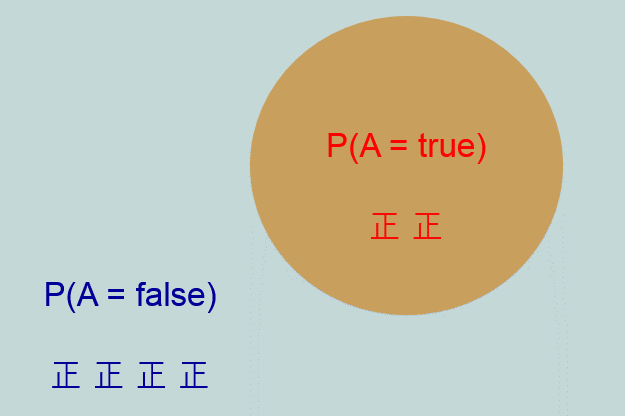
\includegraphics[scale=0.8]{fig7_1.png} 
\caption{사건 $A$의 확률 빈도 그래프}
\label{fig:7-1}
\end{figure} 

\noindent 그림 \ref{fig:7-1}에서 확인할 수 있는 전체 사건의 빈도는 30번이다. 따라서 $A=\textrm{true}$ 사건의 상대 빈도 확률은 $10/(10+20) = 1/3$과 같이 계산할 수 있다. 관측을 아주 많이 해서 확률을 구한다면 확률값은 특정한 숫자에 수렴하게 된다. 그러면 우리는 그것을 $A=\textrm{true}$의 확률이라고 말할 수 있다. \\

%슬라이드 5,6%
\indent 이제는 특정 조건 아래에서의 확률을 나타낼 수 있는 조건부 확률을 생각해 보겠다. 예를 들어, 중간고사에서 70점을 받은 학생의 최종 학점은 무엇일까? 우리는 여기에 대해서 아직 확실한 답을 줄 수 없다. 왜냐하면 최종 학점은 중간고사 점수와 기말고사 점수, 출결 점수를 함께 반영해서 결정하기 때문이다. 그러나 학생이 중간고사에서 70점을 받았다는 것을 알고 있으며, 이러한 사실 아래에서 앞으로의 학점을 확률적으로 예측할 수 있을 것이다. 이러한 관점 아래에서의 확률을 조건부 확률(Conditional Probability)이라고 한다. 여기서는 사건 $A=true$를 "최종 학점으로 A를 받았다.", 사건 $B=true$를 "중간고사에서 70점을 받았다."라고 정의한다면 중간고사에서 70점을 받았을 때 최종 학점으로 A를 받을 확률을 $P(A=true|B=true)$라는 조건부 확률로 표현할 수 있다. 그리고 이 때의 조건부 확률을 $B$라는 조건 아래에서 $A$의 확률(Probability of $A$ conditioned on $B$) 또는 $B$가 주어졌을 때의 $A$의 확률(Probability of $A$ given $B$)이라고 부른다. \\

\begin{figure}[ht] \centering 
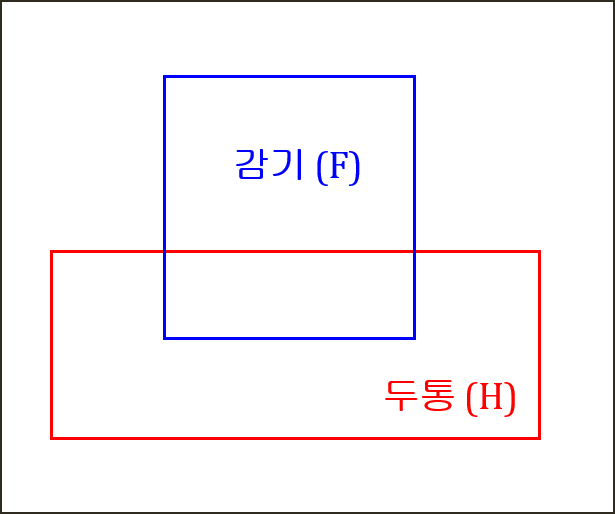
\includegraphics[scale=0.6]{fig7_2.png} 
\caption{두통과 감기 사이의 관계 그래프}
\label{fig:7-2}
\end{figure} 

그림 \ref{fig:7-2}에서는 두통이 왔다는 사건 $H$와 감기에 걸렸다는 사건 $F$를 각각 빨간색 사각형과 파란색 사각형으로 묘사하였다. 여기서 두통이 올 확률은 10\%, 감기에 걸릴 확률은 2.5\%이다. 물론 이것만으로는 두통과 감기 사이의 관계에 대해서 알 수 없다. 그러나 감기에 걸렸을 때 두통이 올 확률이 50\%라고 한다면 조건부 확률에 대한 정보가 주어지면서 두 사건 사이의 관계를 알 수 있다. 여기서 처음에 두통이 올 확률과 감기에 걸릴 확률을 계산하면서 생각한 전체 사건은 그림 \ref{fig:7-2}의 검은색 사각형 전체이다. 하지만 감기에 걸렸을 때 두통이 올 조건부 확률을 계산하면서 생각한 전체 사건은 파란색 사각형의 영역으로 한정된다. 그리고 우리가 고려하는 사건은 빨간색 사각형 전체가 아닌, 파란색 사각형과 빨간색 사각형이 겹치는 영역으로 한정된다. 이것을 수식으로 표현하면 다음과 같다.  
\begin{equation}
P(H|F) = \frac{\textrm{(파란색, 빨간색 사각형이 겹치는 영역)}}{\textrm{(파란색 사각형의 영역)}} = \frac{P(H,F)}{P(F)}
\label{eq:7-1}
\end{equation}
\noindent 여기서 $P(H,F)$는 결합 확률(Joint Probability)이며, 사건 $H$와 사건 $F$가 동시에 일어날 확률을 의미한다. 또한, 수식 (\ref{eq:7-1})은 조건부 확률과 결합 확률 사이의 관계를 나타낸다. \\

%슬라이드 7%
결합 확률은 매우 중요한 개념이다. 결합 확률을 알면 사건의 확률에 대해서 보다 많은 것들을 알 수 있다. 여기서는 먼저 개별 사건의 확률과 결합 확률 사이의 관계를 나타내는 전체 확률의 법칙에 대해서 짚고 넘어가겠다. 전체 확률의 법칙(Law of Total Probability)을 수식으로 나타내면 다음과 같다. 
\begin{equation}
P(A) = \sum_{B} P(A,B)
\label{eq:7-2}
\end{equation}
\noindent 수식 (\ref{eq:7-2})에서는 확률 변수 $B$와 관련된 모든 사건에 대해서 결합 확률 $P(A,B)$를 모두 더해서 $A$의 확률을 구하였다. 이처럼 특정 사건이 일어나는 경우의 결합 확률을 모두 더해서 그 사건이 일어날 확률을 구하는 것을 주변화(Marginalization)라고 한다. 결합 확률을 알면 주변화를 통해서 개별 확률 또한 구할 수 있다. \\

예를 들어, 확률 변수 $A$와 $B$가 각각 true와 false라는 두 가지 값을 가질 수 있다고 하자. 여기서 $A$가 true이려면 $A$와 $B$가 동시에 true이거나, $A$가 true, $B$는 false여야 한다. 이들 두 가지 사건은 동시에 일어날 수 없어 서로 배타적(Exclusive)인 관계이므로, $A$가 true일 확률은 이들 사건의 확률을 더한 값과 같다. 이것을 수식으로 나타내면 다음과 같다.
\begin{equation}
P(A = \mathrm{true}) = P(A = \mathrm{true}, B = \mathrm{true}) + P(A = \mathrm{true}, B = \mathrm{false})
\label{eq:7-3}
\end{equation}

확률 변수가 여러 개인 경우에 대해서도 같은 방법을 적용할 수 있다. 예를 들어, 확률 변수 $A$, $B$, $C$, $D$를 결합한 결합 확률 $P(A,B,C,D)$가 있다면 $B$의 확률은 다음과 같이 결합 확률을 사용해서 다음과 같이 나타낼 수 있다. 
\begin{equation}
P(B) = \sum_{A} \sum_{C} \sum_{D} P(A,B,C,D)
\label{eq:7-5}
\end{equation}

한편, 앞에서 설명한 것처럼 결합 확률과 조건부 확률 사이의 관계를 $P(A|B)=P(A,B)/P(B)$와 같이 수식으로 나타낼 수 있다. 이 수식을 활용해서 전체 확률의 법칙을 다음과 같이 다르게 나타낼 수 있다. 
\begin{equation}
P(A) = \sum_{B} P(A|B)P(B)
\label{eq:7-6}
\end{equation}
\noindent 수식 (\ref{eq:7-6})에서는 개별 사건의 확률을 나타내는데 결합 확률 대신 조건부 확률을 사용했다. 때문에 결합 확률을 모르고 조건부 확률만을 아는 경우에 수식 (\ref{eq:7-6})를 적용할 수 있다. \\

이제 결합 확률로 조건부 확률을 구하는 방법을 생각해 보겠다. 앞에서 보았듯이 결합 확률을 안다면 개별 확률을 계산해서 알 수 있다. 그리고 조건부 확률에 대해서도 결합 확률과 개별 확률을 적절히 활용하여 계산하는 것이 가능하다. 예를 들어, 조건부 확률 $P(C|B)$를 계산한다고 하자. 이 확률은 다음과 같이 $P(A,C,D|B)$를 $A$와 $D$에 대해서 주변화하여 결합 확률만을 사용해서 나타낼 수 있다.   
\begin{equation}
P(C|B) = \sum_{A} \sum_{D} P(A,C,D|B) = \frac{1}{P(B)} \sum_{A} \sum_{D} P(A,B,C,D) 
\label{eq:7-7}
\end{equation}
\noindent 여기서 $1/P(B)$는 정규화 상수(Normalization Constant)이다. 이처럼 결합 확률을 적절히 사용하면 조건부 확률을 구할 수 있다. \\

우리는 결합 확률을 사용해서 개별 확률과 조건부 확률을 각각 구할 수 있다. 또한, 결합 확률로 우리가 생각할 수 있는 모든 사건에 대해서 하나하나 설명할 수 있다. 이처럼 강력한 수단인 결합 확률에는 그러나 치명적인 단점이 있다. 그것은 확률 변수의 개수가 늘어날수록 결합 확률이 다루는 사건의 수가 급격히 늘어난다는 것이다. 예를 들어, 확률 변수 $A$, $B$, $C$, $D$가 각각 true 또는 false를 가진다고 하면 결합 확률이 다루는 사건의 개수는 총 $2^4=16$개가 된다. 여기에 확률 변수 $E$를 추가하면 전체 사건은 $16 \times 2 = 32$개가 되며, $F$를 추가하면 $32 \times 2 = 64$개가 된다. 이처럼 확률 변수가 하나씩 늘어날때마다 전체 사건의 개수는 2배씩 늘어나게 된다. 이런 식으로 필요한 확률 변수의 개수에 대해서 지수적(Exponential) 추세의 증가가 계속된다면 대처하기가 상당히 까다로울 것이다. \\

%슬라이드 8%
이제 결합 확률의 분해에 대해서 생각해 보겠다. 여기서 분해(Factorization)란 결합 확률을 여러 개의 개별 확률과 조건부 확률의 곱으로 나타내는 것을 말한다. 앞에서 결합 확률과 조건부 확률 사이의 관계를 $P(A|B)=P(A,B)/P(B)$와 같은 수식으로 나타낼 수 있다는 것을 배웠다. 이것의 양 변에 $P(B)$를 곱하고 식의 좌우를 바꾸면 다음의 수식이 나온다. 
\begin{equation}
P(A,B) = P(A|B)P(B)
\label{eq:7-8}
\end{equation}
수식 (\ref{eq:7-8})은 두 개의 확률 변수를 가진 결합 확률을 개별 확률과 조건부 확률로 분해한 것과 같다. 여기서는 $A$를 앞에 띄어주고 $A$ 외의 다른 확률 변수인 $B$를 주어진 부분이라고 가정했다. 그리고 주어진 부분인 $P(B)$를 뒤에 따로 기록했다. $A$, $B$, $C$, $\cdots$, $Z$와 같이 수많은 확률 변수가 있는 경우에도 요령은 같다. 
\begin{eqnarray}
P(A, B, C, \cdots, Z) & = & P(A | B, C, \cdots, Z)P(B, C, \cdots, Z) \nonumber \\
& = & P(A | B, C, \cdots, Z) P(B | C, \cdots, Z) P(C, \cdots, Z) \nonumber \\
&  & \cdots \nonumber \\
& = & P(A | B, C, \cdots, Z) P(B | C, \cdots, Z) P(C | \cdots, Z) \cdots P(Z) \nonumber  \\
&  & \label{eq:7-9}
\end{eqnarray}
이런 식으로 결합 확률을 더 이상 나눌 수 없는 개별 확률이 나올 때까지 조건부 확률로 계속해서 분해할 수 있다는 것을 우리는 연쇄 법칙(chain rule)이라고 한다. \\

%슬라이드 9%
결합 확률을 보다 간단히 이해하기 위한 다음의 예시가 있다. 우리는 훌륭한 학자에게는 어떠한 자질이 있는지를 알아보고자 하며, 생각할 수 있는 확률적인 요소에는 학자의 지능 $I$, 노력 $E$, 그리고 대학 시절의 성적 $G$가 있다. 여기서 높은 지능을 가지고 있거나, 노력파이거나, 또는 대학에서 좋은 성적을 받았을 경우에 대해서 $I$, $E$, $G$ 각각에 해당되는 값은 true가 되며, 그렇지 않을 경우에는 false가 된다고 하겠다. 이 때, 각각의 $I$, $E$, $G$값에 대해서 결합 함수값을 다음의 표로 나타낼 수 있다. \\

\begin{figure}[ht] \centering 
\begin{tabular}{|c|c|c|c|}
  \hline
  지능($I$) & 노력($E$) & 성적($G$) & $P(I,E,G)$ \\
  \hline
  true & true & true & 0.15 \\
  \hline
  true & true & false & 0.05 \\
  \hline
  true & false & true & 0.1 \\
  \hline
  true & false & false & 0.3 \\
  \hline
  false & true & true & 0.05 \\
  \hline
  false & true & false & 0.05 \\
  \hline
  false & false & true & 0.2 \\
  \hline
  false & false & false & 0.1 \\ 
  \hline
\end{tabular}
\caption{결합 확률 표}
\label{fig:7-3}
\end{figure} 

여기서 지능과 노력, 그리고 좋은 성적 모두를 겸비한 팔방미인형 학자가 전체에서 차지하는 비율은 10\%밖에 되지 않는다. 그리고 8가지 서로 다른 유형의 결합 확률을 합한 값은 반드시 1이 되어야 한다. 여기서 똑똑한 학자의 비율은 어떻게 될까? 이 경우, 그림 \ref{fig:7-3}의 표에서 $I$가 true인 경우의 모든 결합 확률을 더해서 그 값을 알 수 있다. 여기서는 $0.15+0.05+0.1+0.3=0.6$이 된다. 다시 말해, $I=\textrm{true}=0.6$이다. 대학 성적이 좋았던 학자들 중 똑똑하면서 노력파인 학자의 비율은 어떻게 될까? 다시 말해, $P(I=\textrm{true}, E=\textrm{true} \ | \ G=\textrm{true})$는 얼마일까? 조건부 확률의 정의에 따라서 우리는 $P(I=\textrm{true}, E=\textrm{true}, G=\textrm{true})$와 $P(G=\textrm{true})$만을 구하면 된다. 첫 번째 확률값은 첫 번째 $P(I,E,G)$의 $0.15$이다. 두 번째 확률값은 첫 번째, 세 번째, 다섯 번째, 일곱 번째 $P(I,E,G)$의 값을 모두 더한 $0.5$이다. 이제 첫 번째 값에 두 번째 값을 나눠서 최종 확률값인 $0.15/0.5 = 0.3$을 구하면 된다. \\

%-----------------------------------------------------------------
\subsection{독립과 조건부 독립}
%-----------------------------------------------------------------

%슬라이드 10%
우리는 결합 확률과 조건부 확률에 대해서 독립(Independence)이라는 개념을 정의할 수 있다. 다음과 같이 결합 확률을 개별 확률의 곱으로 나타낼 수 있다면 두 사건은 서로 독립이다. 
\begin{equation}
P(A,B) = P(A)P(B)
\label{eq:7-10}
\end{equation}
또한, 다음과 같이 조건부 확률이 개별 확률과 같다면 두 사건은 역시 서로 독립이다. 
\begin{equation}
P(A|B) = P(A)
\label{eq:7-11}
\end{equation}
결합 확률과 조건부 확률 사이에는 밀접한 관계가 있으므로 수식 (\ref{eq:7-10})와 수식 (\ref{eq:7-11})은 모두 사건 $A$와 사건 $B$가 독립이라는 것을 말하고 있다. \\

Chapter 1에서 배운 압정 던지기로 독립 개념을 이해해보자. 처음 압정을 던져서 위가 나왔다고 해서 다음 던지는 압정이 다시 위가 나올 확률이 높다고 할 수는 없다. 다시 말해, 첫 번째 압정을 던지는 것과 두 번째 압정을 던지는 것은 아무런 관계가 없으며, 서로 독립이라고 할 수 있다. 세 번째, 네 번째, 심지어는 $n$번째로 던지는 압정에 대해서도 이것은 마찬가지이다. 때문에 압정을 $n$번 던졌을때 모두 위가 나올 확률을 구하기 위해서는 그것에 해당되는 결합 확률을 찾는 대신 첫 번째, 두 번째, $\cdots$, $n$번째에 대해서 개별 확률을 찾아서 모두 곱하는 것으로 충분하다. 이것을 수식으로 나타내면 다음과 같다.
\begin{equation}
P(C_1,\cdots,C_n) = \prod_{i=1}^{n} P(C_i)
\label{eq:7-12}
\end{equation} \\

%슬라이드 11%
독립에는 주변 독립(Marginal Independence)과 조건부 독립(Conditional Independence)이라는 두 가지 종류가 있다. 주변 독립은 앞에서 설명한 독립의 정의와 완전히 동일하므로 이전처럼 독립이라고 표현해도 무방하다. 반면에, 조건부 독립은 주변 독립과는 다른 개념이며 베이지안 네트워크를 이해하는데 있어서 중요한 역할을 한다. \\

조건부 독립은 다음과 같다. 사건 $C$가 이미 주어진 상황에서 사건 $A$와 사건 $B$가 서로 독립인 상황을 조건부 독립이라고 한다. 이것을 수식으로 나타내면 다음과 같다. 
\begin{equation}
P(A|B,C) = P(A|C)
\label{eq:7-13}
\end{equation}
여기서 중요한 것은 사건 $A$와 사건 $B$가 독립이 아니더라도 ($P(A|B) \neq P(A)$),  사건 $C$가 주어진 상황에서 조건부 독립일 수 있다는 것이다. \\

\begin{figure}[ht] \centering 
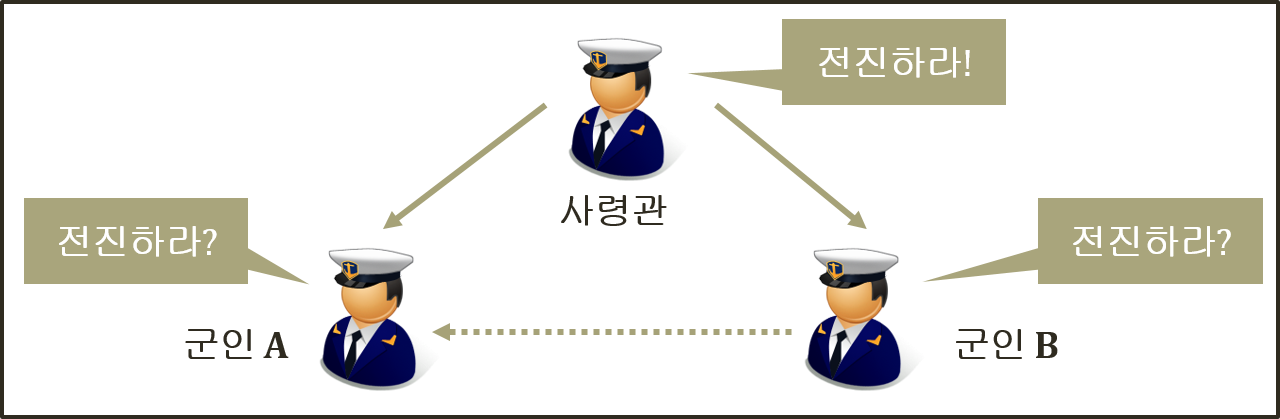
\includegraphics[scale=0.45]{fig7_4.png} 
\caption{명령 체계}
\label{fig:7-4}
\end{figure} 

예를 들어, 그림 \ref{fig:7-4}에서와 같이 두 군인 $A$, $B$가 사령관 $C$로부터 명령을 받는 상황이다. 사령관이 전진하라고 명령하면 군인인 $A$, $B$는 명령에 따라서 전진해야 한다. 여기서 $A$의 무전기가 고장나서 사령관의 명령을 듣지 못하는 상황이라고 하자. 그러한 상황에서 $A$는 $A$ 앞에 있는 $B$가 전진하는 것을 보면서 같이 전진한다. 그리고 $B$가 행군을 멈추면 $A$도 같이 멈춘다. 이 때, $B$의 행동은 $A$의 행동에 영향을 미치므로 이들은 독립 관계가 아닌 것이 된다. 그러나 $A$가 무전기를 고치고 나면 이제 $A$의 행동은 사령관 $C$의 명령을 받아서 결정된다. 그 때문에 더 이상 $B$에 대한 정보에는 신경을 쓰지 않게 된다. 즉, $C$의 명령이라는 것이 특정한 이벤트로 주어진 상황에서 다른 이벤트인 $B$의 행동과는 독립 관계가 되는 것이다. 이렇게 $C$의 명령이라는 조건이 붙은 독립이 바로 조건부 독립이다. 

%-----------------------------------------------------------------
\section{베이지안 네트워크}
%-----------------------------------------------------------------

%-----------------------------------------------------------------
\subsection{베이지안 네트워크}
%-----------------------------------------------------------------

%슬라이드 12,13%
이제는 베이지안 네트워크를 소개하고 문법과 의미(semantics)가 어떻게 되는지를 알아보겠다. \\

우리는 chapter 3에서 나이브 베이즈를 다루었다. 나이브 베이즈의 목적은 다음의 나이브 베이즈 함수를 최대로 만드는 파라미터 $y$를 찾는 것이 된다.
\begin{equation}
f_{NB}(x) = \textrm{argmax}_{Y=y} \ P(Y=y) \ \prod_{i=1}^{d} P(X_i = x_i \ | \ Y=y)
\label{eq:7-14}
\end{equation} 
여기서는 나이브 가정에 따라 $Y=y$가 주어진 상황에서 개별 $X_i$가 서로 독립임을 가정하므로, $X_i$와 $Y$ 사이의 관계를 그림 \ref{fig:7-5}와 같이 나타낼 수 있다.
\begin{figure}[ht] \centering 
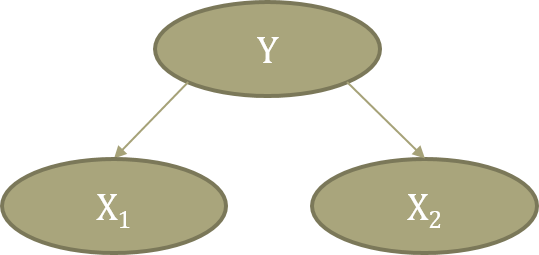
\includegraphics[scale=0.6]{fig7_5.png} 
\caption{나이브 베이지안 네트워크}
\label{fig:7-5}
\end{figure} 
그림 \ref{fig:7-5}에서의 노드는 하나의 확률 변수를 의미하며, $Y$와 각 $X_i$ 사이의 관계를 화살표로 나타내었다. $X_1$과 $X_2$ 사이에 화살표가 없는데 여기에는 조건부 독립을 가정했기 때문이다. 이처럼, 나이브 베이즈 모델을 간단하게 나타낼 수 있다. 그렇다면 보다 복잡한 모델에 대해서는 어떨까? 우리는 베이지안 네트워크를 여기에 적용할 수 있다.\\

%슬라이드 14%
베이지안 네트워크(Bayesian Network)는 그래픽 표기법(Graphical Notation)의 하나로서, 확률 변수와 확률 변수 사이의 조건부 독립 관계에 대해서 말하고 있다. 또한, 베이지안 네트워크는 확률 변수의 결합 확률 분포를 가장 확실히 나타낼 수 있는 표현 방법이다. \\ 

우리는 베이지안 네트워크의 문법(Syntax)에 대해서 알아야 한다. 베이지안 네트워크에서 사용하는 그래프는 비순환 방향 그래프(Acyclic Directed Graph)이다. 여기서 "비순환"은 그래프에 사이클(Cycle)이 없다는 것을 말하며, "방향"은 노드와 노드를 연결하는 아크에 방향이 있다는 것을 말한다. 노드(Node)는 하나의 확률 변수를 의미한다. 아크(Arc)는 확률 변수 사이의 종속 관계를 의미하며, 화살표가 나오는 노드의 확률 변수에 의해서 화살표가 가리키는 노드의 확률 변수가 영향을 받음을 말해준다. \\

예를 들어, 그림 \ref{fig:7-5}에서 $X_1$과 $X_2$의 부모 노드는 $Y$이므로, $X_1$과 $X_2$는 $Y$의 영향을 받는다. 이것을 확률적인 의미에서 보면 $X_1$ 노드는 $P(X_1|Y)$ 확률을, $X_2$ 노드는 $P(X_2|Y)$ 확률을 표현하고 있다. 물론 $Y$에는 부모 노드가 없으므로 $Y$ 그대로 $P(Y)$로 나타내거나, 또는 전체 사건인 $\Omega$를 사용해서  $P(Y|\Omega)$로 표현할 수 있다. \\

\begin{figure}[ht] \centering 
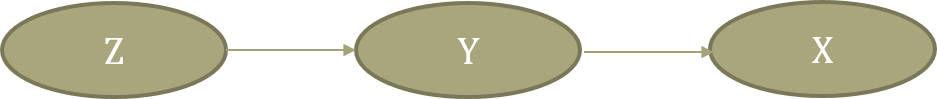
\includegraphics[scale=0.6]{fig7_6.png} 
\caption{간접 영향}
\label{fig:7-6}
\end{figure} 

한편, 여기에는 아크로 직접 표현하는 직접 영향(Direct Influence) 외에 간접 영향(Indirect Influence)이 있다. 그림 \ref{fig:7-6}에 따르면 $Z$는 $Y$에, $Y$는 $X$에 영향을 주고 있다. 여기서 $Z$는 $X$와 아크로 직접 연결되어 있지는 않지만 $X$에 간접적인 영향을 주게 된다. \\

%슬라이드 15%
지금까지의 설명으로 이제는 우리가 직접 베이지안 네트워크를 그릴 수 있을 것이다. 다음의 예시를 생각해 보자. 입 안에 충치가 생기면 이빨이 아프고 입에서 냄새가 나며, 이러한 상황은 지금의 날씨와는 아무런 관계가 없다. 이것을 베이지안 네트워크로 나타내면 다음과 같다.  \\
\begin{figure}[ht] \centering 
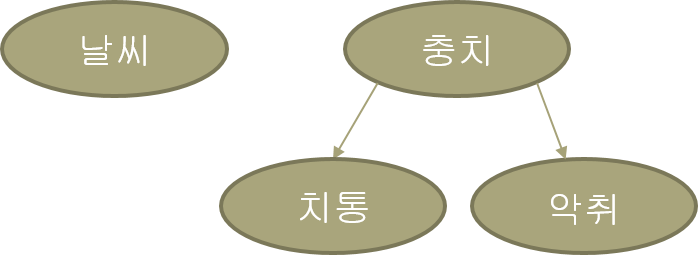
\includegraphics[scale=0.6]{fig7_7.png} 
\caption{베이지안 네트워크 예시}
\label{fig:7-7}
\end{figure} 

\noindent 이 베이지안 네트워크를 역으로 해석하면, 날씨는 다른 변수와 연결되어 있지 않으므로 다른 변수에 대해서 독립이다. 한편, 충치가 있을 때 이빨이 아프다면 냄새가 날 확률 또한 올라가며, 반면에 충치가 없다면 이빨이 아픈 것은 냄새가 나는 것에 영향을 주지 않는다. 다시 말해, 이빨이 아픈 것과 냄새가 나는 것이 서로 독립인지 아닌지는 충치가 있을 때와 없을 때가 다른 것이다. 때문에 이빨이 아픈 것과 입에서 냄새가 나는 것은 충치가 없다는 정보 아래에서 조건부 독립이다. \\

여기에 나이라는 요소를 추가해 보자. 전문가에 따르면 나이를 먹을수록 충치가 더 잘 생길수 있다고 한다. 여러분은 나이와 충치 사이의 관계라는 새로운 정보를 그림 \ref{fig:7-7}의 베이지안 네트워크에 추가할 수 있다. \\

\begin{figure}[ht] \centering 
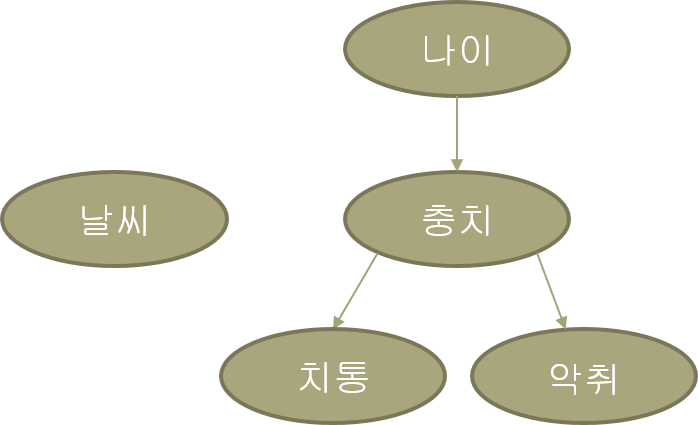
\includegraphics[scale=0.6]{fig7_7_1.png} 
\caption{나이가 추가된 베이지안 네트워크 예시}
\label{fig:7-7-1}
\end{figure} 

\noindent 그림 \ref{fig:7-7-1}의 새로운 베이지안 네트워크에 따르면 나이와 충치 사이에는 직접적인 관계가 있다. 한편, 나이가 많으면 충치가 생길 확률이 높아지며, 충치가 생길 확률이 높으며 이빨이 아프거나 냄새가 날 수 있다. 따라서 나이가 많다는 사실은 각각 이빨이 아픈 것, 냄새가 나는 것에 간접적인 영향을 준다고 할 수 있게 된다. \\

%슬라이드 16%
이제는 조금 더 어려운 예제를 생각해 보겠다. 다음의 예제는 왠만한 기계 학습 강의에서 다루고 있는 전통적으로 유명한 예제이다. 이 예제에서 여러분은 단독 주택에 살고 있으며, 양 옆집에는 존과 메리가 살고 있다. 단독 주택에는 도둑이 들기 쉽기 때문에 여러분은 도둑이 들면 알람이 울리는 센서를 설치했다. 센서에서 알람이 울리면 존이 나에게 전화를 하기도 하고 메리가 여러분에게 전화를 하기도 한다. (즉, 여러분은 직접 알람 소리를 들을 수 없다.) 그런데 센서가 그렇게 정확하지 않아서 도둑이 들었을 때가 아니라 지진이 났을 때에도 알람이 울릴 수 있다. \\

여기서 직접 영향의 관계에 있는 사건들을 살펴보도록 하겠다. 도둑이 든 것, 지진이 발생한 것과 알람이 울리는 것에는 직접적인 연관이 있다. 도둑($B$), 지진($E$)은 알람($A$)의 행동에 직접 영향을 주고 있는 것이다. 또한, 알람이 울리는 것과 존, 메리가 각각 나에게 전화를 하는 것에는 직접적인 연관이 있다. 알람($A$)은 존($J$), 메리($M$)의 행동에 직접 영향을 주고 있는 것이다. 지금가지의 설명을 베이지안 네트워크로 표현하면 다음과 같다. \\

\begin{figure}[ht] \centering 
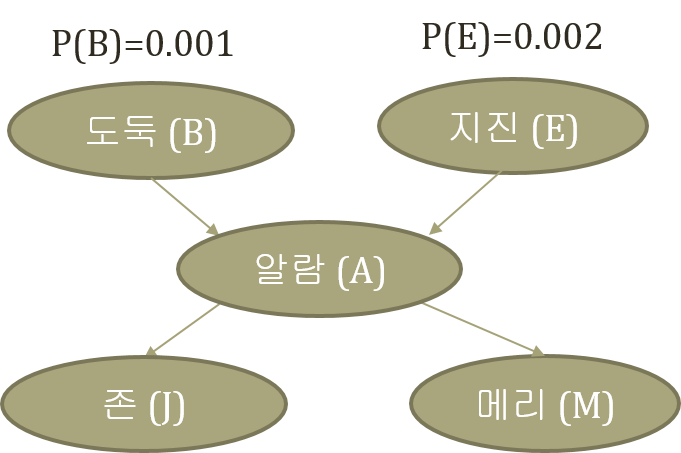
\includegraphics[scale=0.6]{fig7_8.png} 
\caption{시나리오에 대한 베이지안 네트워크 예시}
\label{fig:7-8}
\end{figure} 

여기서 도둑이 들 확률은 $P(B)=0.001$, 지진이 발생할 확률은 $P(E)=0.002$이다. 그림 \ref{fig:7-8}에 나오는 것처럼 $B$와 $E$에는 사전 조건이 될 부모 노드가 없으므로 이와 같이 하나의 숫자로 표현할 수 있다. 한편, 서로 영향을 주고 받는 사건들 사이의 확률 관계는 다음의 조건부 확률 표로 나타낼 수 있다. \\

\begin{figure}[ht] \centering 
\parbox[t]{3cm}
{
\begin{tabular}{|c|c|c|}
  \hline
  도둑($B$) & 지진($E$) & $P(A|B,E)$ \\
  \hline
  true & true & 0.95 \\
  \hline
  true & false & 0.94 \\
  \hline
  false & true & 0.29 \\
  \hline
  false & false & 0.001 \\
  \hline
\end{tabular}
} \hspace{3cm}
\parbox[t]{5cm}
{
\begin{tabular}{|c|c|c|}
  \hline
  알람($A$) & $P(J|A)$ & $P(M|A)$ \\
  \hline
  true & 0.90 & 0.70 \\
  \hline
  false & 0.05 & 0.01 \\
  \hline
\end{tabular}
}
\caption{조건부 확률 표}
\label{fig:7-9}
\end{figure} 

그림 \ref{fig:7-9}의 왼쪽 표에서는 도둑이 들었으면서 동시에 지진이 발생했을 때, 알람이 울릴 확률이 0.95라는 것을 알 수 있으며 그 외의 경우에 대해서도 마찬가지로 확인할 수 있다. 또한, 그림 \ref{fig:7-9}의 오른쪽 표에서는 알람이 울렸을 때, 존이 나에게 전화를 할 확률이 0.9, 메리가 나에게 전화를 할 확률이 0.7이라는 것을 알 수 있다. \\

%슬라이드 17%
이처럼 베이지안 네트워크는 개별 시나리오에 대한 전반적인 지식을 나타낸다. 그리고 이러한 지식은 질적 구성요소와 양적 구성요소로 구분할 수 있다. 먼저 질적 구성요소(Qualitative Components)로는 상관관계에 대한 사전 지식, 주어진 데이터로부터의 학습, 전문 지식이나 상식, 위상적 구조에 대한 고려 등이 있다. 그리고 양적 구성요소(Quantitative Components)로는 이산 확률 변수의 경우에는 조건부 확률 표가, 연속 확률 변수의 경우에는 확률 분포 함수가 있을 수 있다. 존이나 메리가 나에게 전화를 했다는 사실이 주어진 상황에서 도둑이 들었을 확률이 얼마인지를 판단하기 위해서는 이러한 질적 구성요소와 양적 구성요소를 동시에 활용할 수 있어야 한다. \\

%슬라이드 22%
\begin{figure}[ht] \centering 
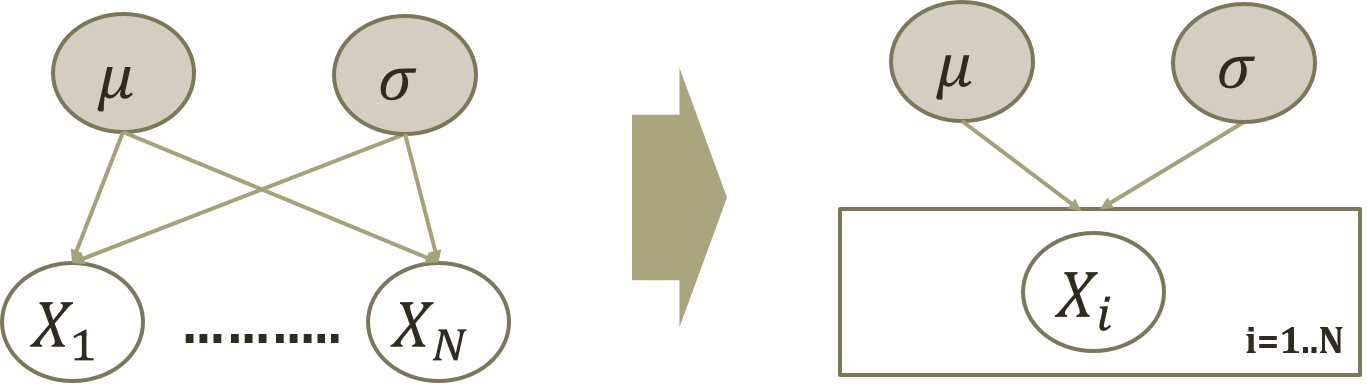
\includegraphics[scale=0.45]{fig7_15.png} 
\caption{판 표기법 예시}
\label{fig:7-13-1}
\end{figure} 

마지막으로 베이지안 네트워크의 표기에 대해서 하나만 더 알아보겠다. 베이지안 네트워크를 더욱 간단히 나타내기 위한 표기법으로 판 표기법(Plate Notation)이 있다. 예를 들어, 그림 \ref{fig:7-13-1}에서와 같이 $\mu$와 $\sigma$라는 파라미터가 $X_1,$ $\cdots,$ $X_N$에 연결되어 있다면 노드 사이의 관계를 표현하기 위해서 모두 $2N$개의 아크를 표시해야 한다. 그러나 이것을 모두 표시하면 전체 네트워크는 번잡해 보인다. 따라서 그 대신 판을 하나 만들어서 판 위에 $X_i$라는 노드를 표시하고 이것으로 $X_1,$ $\cdots,$ $X_N$의 모든 노드를 표현했다고 여기는 것이다. 또한 판 표기법에서는 판 안의 모든 변수가 독립 동일 분포(Independent and Identically Distribution)라는 나이브한 가정을 포함하고 있으므로 전체 확률식을 다음과 같이 분해할 수 있다.
\begin{equation}
P(X_1,\cdots,X_N | \ \mu,\sigma) = \prod_{n=1}^{N} P(X_n| \ \mu,\sigma)
\label{eq:7-13-2}
\end{equation}
텍스트 마이닝(Text Mining)에서는 여러 개의 확률 변수가 공통 파라미터를 가지는 경우가 많으므로 이러한 표기법을 자주 사용한다. \\ 

%-----------------------------------------------------------------
\subsection{베이즈 볼 알고리즘}
%-----------------------------------------------------------------

%슬라이드 18%
이제 큰 규모의 베이지안 네트워크를 분석하는 방법을 알아보겠다. 베이지안 네트워크의 세부 구조에는 다음의 세 가지 일반적인 형태가 있다. \\

\begin{figure}[ht] \centering 
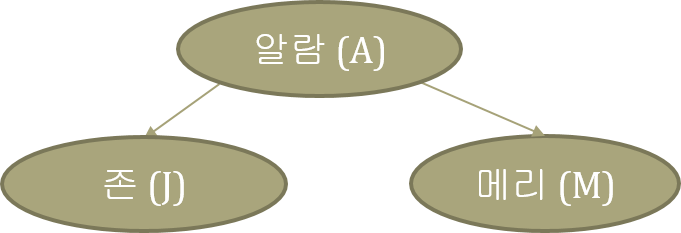
\includegraphics[scale=0.6]{fig7_8_1.png} 
\caption{공통 부모 관계}
\label{fig:7-8-1}
\end{figure} 

첫 번째 형태는 두 노드가 공통의 부모(Common Parent)를 가지는 경우이다. 그림 \ref{fig:7-8-1}의 베이지안 네트워크가 이러한 관계를 나타내며, $J \bot M | A$라고 표기할 수 있다. 이것은 $A$가 주어졌을 때 $A$로부터 영향을 받는 $J$와 $M$이 조건부 독립 관계에 있다는 가장 대표적인 경우를 의미한다. 수식으로 나타내면 $P(J,M|A)=P(J|A)P(M|A)$와 같다. \\

\begin{figure}[ht] \centering 
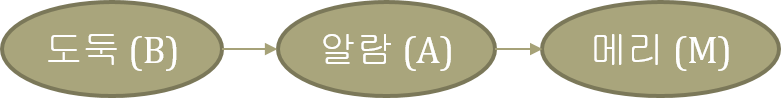
\includegraphics[scale=0.6]{fig7_8_2.png} 
\caption{연속 관계}
\label{fig:7-8-2}
\end{figure} 

두 번째 형태는 세 노드가 차례대로 연결되어 있는 연속(Cascading) 관계의 경우이다. 그림 \ref{fig:7-8-2}의 베이지안 네트워크가 이러한 관계를 나타내며, 이것을 $B \bot M | A$라고 표기할 수 있다. 연속 관계는 가운데의 $A$가 주어졌을 때 $A$에 영향을 주는 $B$와 $A$로부터 영향을 받는 $M$이 조건부 독립 관계에 있다는 경우를 의미한다. 예를 들어, 알람이 울렸는지를 안다면 메리가 전화를 할 확률을 정확히 알 수 있으며, 이러한 상황에서 도둑이 왔는지 오지 않았는지는 중요하지 않게 되는 것이다. 이것을 수식으로 나타내면 $P(M|B,A)=P(M|A)$와 같다. \\

\begin{figure}[ht] \centering 
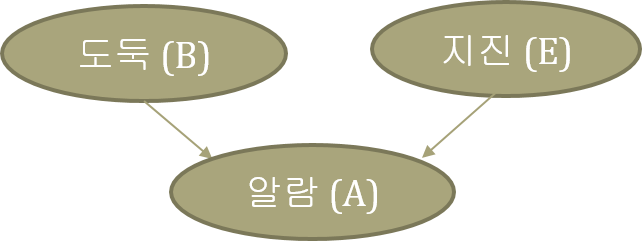
\includegraphics[scale=0.6]{fig7_8_3.png} 
\caption{V-구조 관계}
\label{fig:7-8-3}
\end{figure} 

세 번째 형태는 두 부모 노드가 공통의 자식을 가지는 V-구조(V-Structure) 관계의 경우이다. 그림 \ref{fig:7-8-3}의 베이지안 네트워크가 이러한 관계를 나타내며, 이것을 $\sim(B \bot E | A)$라고 표기할 수 있다. V-구조 관계는 $A$가 주어지지 않았을 경우에 $B$와 $E$가 독립이라는 것을 의미하며 반대로 $A$가 주어지면 $B$와 $E$는 더 이상 독립 관계에 있지 않게 되는 경우이다. 이전까지와는 상황이 정반대이므로 이해하는데 있어서 세심한 주의가 필요하다. 예를 들어, 알람이 울렸는지 모르는 상황에서 지진이 일어나는 것과 도둑이 드는 것은 아무런 관계가 없다. 그러나 알람이 울린 상황에서 지진이 발생하지 않았다면 우리는 이것이 높은 확률로 도둑이 들어왔기 때문이라고 추측할 수 있다. 다시 말해, 알람이 울렸다는 정보를 알고 있는 상황에서는 지진이 발생했다는/발생하지 않았다는 정보가 도둑이 들었다는/들지 않았다는 정보에 영향을 미치게 되는 것이다. 이것을 수식으로 나타내면 $P(B,E,A) = P(B) P(E) P(A|B,E)$와 같다. \\

%슬라이드 19%
우리가 베이지안 네트워크를 분석할 때에 조건부 독립 정보를 아는 것은 중요하다. 왜냐하면 사전에 주어진 조건부 독립 정보를 활용하면 결합 확률을 분해한 식이 훨씬 간단해지기 때문이다. 베이지안 네트워크가 있을 때 확률 변수들 사이의 조건부 독립 관계를 알 수 있는 알고리즘으로 베이즈 볼 알고리즘(Bayes Ball Algorithm)이 있다. 이 알고리즘은 몇몇 확률 변수의 정보가 사전에 주어졌을 때, 정해진 확률 변수에서 시작해서  규칙에 따라 다른 확률 변수로 공을 굴릴 수 있는지로 두 확률 변수가 독립인지를 확인해 주는 알고리즘이다. 여기에는 베이지안 네트워크의 세부 구조와 사전에 알려진 확률 변수의 정보에 따른 알고리즘의 규칙이 있다. \\ 

\begin{figure}[ht] \centering 
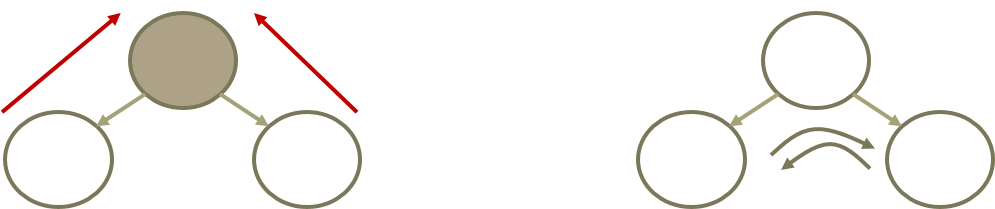
\includegraphics[scale=0.6]{fig7_10_2.png} 
\caption{공통 부모 관계에서의 베이즈 볼}
\label{fig:7-10-2}
\end{figure} 

그림 \ref{fig:7-10-2}에서와 같이 두 노드가 공통의 부모를 가지는 경우에 베이즈 볼은 다음과 같은 규칙으로 굴러간다. 왼쪽 그래프에서처럼 부모 노드의 정보를 알고 있다면 더 이상 베이즈 볼이 굴러갈 수 없어 이들 자식 노드에 각각 해당되는 두 변수는 서로 독립이다. 그러나 오른쪽 그래프에서처럼 부모 노드의 정보를 모른다면 두 자식 노드 사이로 베이즈 볼이 자유롭게 굴러갈 수 있어 두 변수 사이는 독립 관계가 아니다.  \\ 

\begin{figure}[ht] \centering 
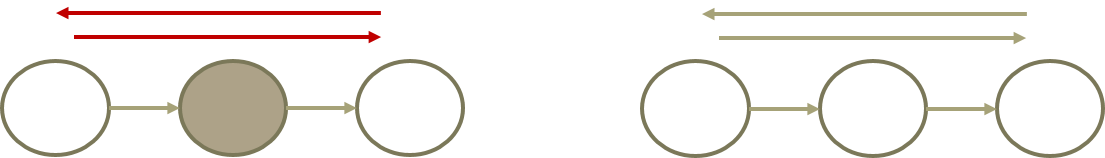
\includegraphics[scale=0.6]{fig7_10_1.png} 
\caption{연속 관계에서의 베이즈 볼}
\label{fig:7-10-1}
\end{figure} 

그림 \ref{fig:7-10-1}에서와 같이 차례대로 연결되어 있는 연속 관계의 경우에 베이즈 볼은 다음과 같은 규칙으로 굴러간다. 왼쪽 그래프에서처럼 두 번째 노드의 정보를 알고 있다면 두 번째 노드를 거쳐서 첫 번째 노드에서 세 번째 노드로, 세 번째 노드에서 첫 번째 노드로 공을 굴릴 수 없다. 따라서 첫 번째 노드에 해당되는 변수와 세 번째 변수에 해당되는 변수는 서로 독립이다. 그러나 오른쪽 그래프에서처럼 두 번째 노드의 정보를 모른다면 첫 번째 노드와 세 번째 노드 사이에서 베이즈 볼은 자유롭게 굴러갈 수 있어 두 변수는 독립 관계가 아니다. \\ 

\begin{figure}[ht] \centering 
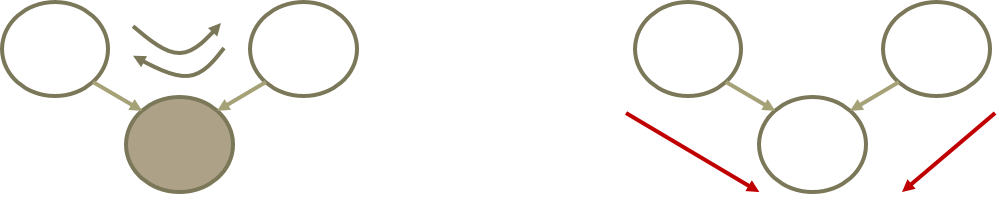
\includegraphics[scale=0.6]{fig7_10_3.png} 
\caption{V-구조 관계에서의 베이즈 볼}
\label{fig:7-10-3}
\end{figure} 

그림 \ref{fig:7-10-3}에서와 같이 두 부모 노드가 공통의 자식을 가지는 V-구조 관계의 경우 베이즈 볼은 공통 부모 관계와는 정 반대의 규칙으로 굴러간다. 왼쪽 그래프에서처럼 부모 노드의 정보를 알고 있다면 두 자식 사이로 베이즈 볼이 자유롭게 굴러갈 수 있어 두 변수 사이는 독립 관계가 아니다. 그러나 오른쪽 그래프에서처럼 부모 노드의 정보를 모른다면 두 자식 사이로 베이즈 볼이 굴러갈 수 없어 두 변수는 서로 독립이다. \\ 

\begin{figure}[ht] \centering 
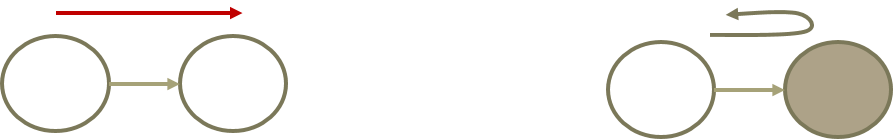
\includegraphics[scale=0.6]{fig7_10_4.png} 
\caption{부모 노드가 없는 경우의 베이즈 볼}
\label{fig:7-10-4}
\end{figure} 

{\color{red} 앞의 세 경우와는 다르게 단 하나의 노드와 연결되어 있는 경우에 대해서도 베이즈 볼 알고리즘의 규칙을 세울 수 있다. 먼저 그림 \ref{fig:7-10-4}에서 베이즈 볼을 굴리기 시작한 노드의 자식 노드가 고립되어 있는 경우를 보자. 왼쪽 그래프에서 시작 노드에는 부모가 없어 다른 노드에 의해서 그것의 정보가 결정되지 않기 때문에 네트워크의 나머지 노드들과는 조건부 독립이다. 따라서 베이즈 볼을 자식 노드로 굴릴 수 없다. 그러나 오른쪽 그래프에서와 같이 자식 노드에 대한 정보가 알려져 있다면, 자식 노드의 정보를 통해서 시작 노드의 정보를 추측할 수 있다. 따라서 베이즈 볼을 자식 노드로 굴릴 수 있다.} \\

\begin{figure}[ht] \centering 
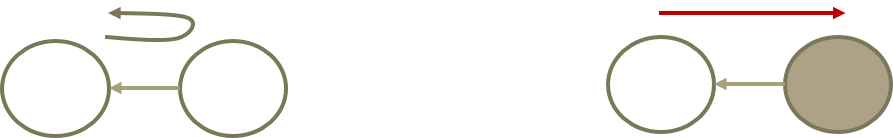
\includegraphics[scale=0.6]{fig7_10_5.png} 
\caption{자식 노드가 없는 경우의 베이즈 볼}
\label{fig:7-10-5}
\end{figure} 

{\color{red}  다음으로 그림 \ref{fig:7-10-5}에서처럼 베이즈 볼을 굴리기 시작한 노드의 부모 노드가 고립되어 있는 경우를 보자. 왼쪽 그래프에서 시작 노드는 그것의 부모 노드와 직접적인 연관 관계가 있다. 따라서 베이즈 볼을 부모 노드로 굴릴 수 있다. 그러나 오른쪽 그래프에서와 같이 부모 노드에 대한 정보가 알려져 있다면, 시작 노드는 오로지 부모 노드와만 직접적인 관계를 가지며 부모 노드 너머의 노드와는 조건부 독립이 된다. 다라서 베이즈 볼을 부모 노드로 굴릴 수 없다.} \\

%슬라이드 20%
\begin{figure}[ht] \centering 
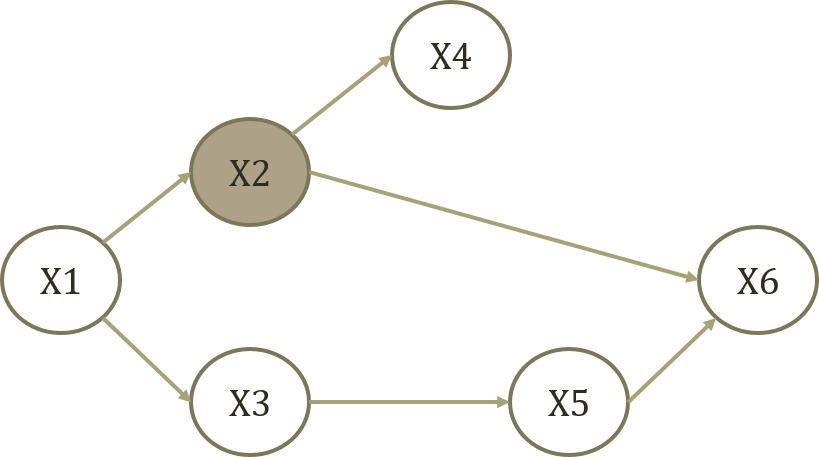
\includegraphics[scale=0.45]{fig7_11_1.png} 
\caption{베이즈 볼 알고리즘 예제 1}
\label{fig:7-11-1}
\end{figure} 

그림 \ref{fig:7-11-1}의 예제로 베이즈 볼 알고리즘의 과정을 살펴볼 수 있다. 여기에는 베이즈 네트워크가 있으며, 사전에 $X_2$의 정보가 주어져 있다. 여기서 $X_1$, $X_4$가 독립인지 확인해 보자. 먼저 $X_1$에서 시작해서 $X_1$, $X_2$, $X_4$가 연속 관계이며, 가운데의 $X_2$에 대한 정보를 알고 있다. 따라서 베이즈 볼은 $X_1$에서 $X_2$를 거쳐 $X_4$로 굴러갈 수 없다. 이번에는 $X_1$에서 시작해서 $X_1$, $X_3$, $X_5$가 연속 관계이며, 가운데의 $X_3$에 대한 정보를 모르고 있다. 따라서 베이즈 볼은 $X_1$에서 $X_3$을 거쳐 $X_5$로 굴러갈 수 있다. 다음으로 $X_5$, $X_6$, $X_2$는 V-구조 관계이며, 공통 자식인 $X_6$의 정보를 모르고 있다. 따라서 따라서 베이즈 볼은 $X_5$에서 $X_6$을 거쳐 $X_2$로 굴러갈 수 없다. 결론적으로, $X_1$에서 시작해서 $X_4$로 향하는 모든 길이 막혔으므로 $X_1$과 $X_4$는 $X_2$의 정보가 주어진 상황에서의 조건부 독립이다. \\

\begin{figure}[ht] \centering 
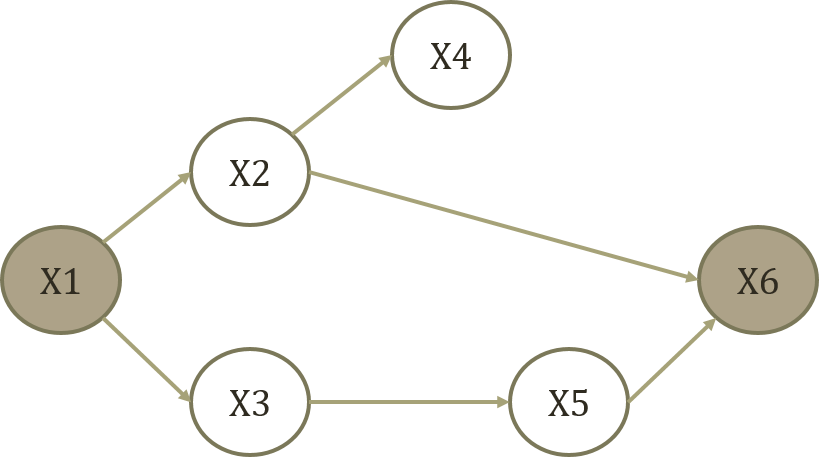
\includegraphics[scale=0.45]{fig7_11_2.png} 
\caption{베이즈 볼 알고리즘 예제 2}
\label{fig:7-11-2}
\end{figure} 

베이즈 볼 알고리즘을 보다 구체적으로 이해하기 위해서 예제를 하나 더 살펴보겠다. 그림 \ref{fig:7-11-2}의 예제는 이전과 네트워크 구조는 동일하지만 사전에 정보가 주어진 확률 변수가 $X_1$, $X_6$으로 이전과는 다르다. 여기서 $X_2$, $X_3$가 독립인지 확인해 보자. 먼저 $X_2$에서 시작해서 $X_2$, $X_6$, $X_5$가 V-구조 관계이며, 공통 자식인 $X_6$에 대한 정보를 알고 있다. 따라서 베이즈 볼은 $X_2$에서 $X_6$, $X_5$로 굴러갈 수 있다. 다음으로 $X_6$에서 시작해서 $X_6$, $X_5$, $X_3$가 연속 관계이며, 가운데의 $X_5$에 대한 정보를 모르고 있다. 따라서 베이즈 볼은 $X_5$에서 $X_6$, $X_3$으로 굴러갈 수 있다. 결론적으로, $X_2$에서 시작해서 $X_3$로 베이즈 볼이 굴러갈 수 있으므로 $X_2$ $X_1$, $X_6$의 정보가 주어진 상황에서 $X_3$는와 조건부 독립이 아니다. \\

\begin{figure}[ht] \centering 
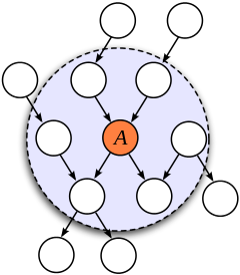
\includegraphics[scale=0.8]{fig7_12.png} 
\caption{베이즈 볼 알고리즘 예제 2}
\label{fig:7-12}
\end{figure} 

이제 V-구조까지 이해했다면 D-분리(D-Seperation)과 마코프 블랭킷을 제대로 정의할 수 있다. 먼저 마코프 블랭킷을 이해하기 위해서 그림 \ref{fig:7-12}의 베이지안 네트워크를 보자. 이 베이지안 네트워크에는 $A$와 그 외 12개의 확률 변수가 아크에 의해서 연결되어 있다. 여기서 노드 $A$의 부모 노드, 자식 노드, 자식 노드의 다른 부모 노드를 모두 묶어서 하나의 동그라미 안에 넣는다. 그러면 동그라미 안의 여섯 개의 확률 변수에 대해서만 알면 나머지 여섯 개의 확률 변수는 $A$와 조건부 독립이 된다. 이 때, $A$를 포함해서 동그라미 안의 노드를 모두 묶은 것을 마코프 블랭킷(Markov Blanket)이라고 부른다. 수식으로 나타내면, 
\begin{equation}
P(A | \mathrm{blanket}, B) = P(A | \mathrm{blanket})
\label{eq:7-13-3}
\end{equation}
와 같으며, 이를 $A \perp B | \mathrm{blanket}$으로 표기한다. 마코브 블랭킷의 기본 원리는 다음과 같다. 우선 노드 $A$의 부모 노드와 자식 노드는 그림 \ref{fig:7-10-3}의 왼쪽 그래프에서처럼 연속 관계에 의해서 베이즈 볼이 굴러가는 것을 막아준다. 그리고 $A$의 자식 노드의 다른 부모 노드는 그림 \ref{fig:7-10-1}의 오른쪽 그래프에서처럼 V-구조 관계에 의해서 베이즈 볼이 굴러가는 것을 막아준다. \\

또한, 사전 정보 $Y$가 주어진 상황에서 베이지안 네트워크의 노드 집단 $X$의 노드에서 노드 집단 $Z$의 노드로 베이즈 볼을 굴릴 수 없다면, $Y$가 주어졌을 때 $X$가 $Z$로부터 D-분리(D-Seperation)되었다고 말한다. 여기서 D-분리의 D는 '직접(Directed)'을 의미한다.

%-----------------------------------------------------------------
\section{베이지안 네트워크의 활용}
%-----------------------------------------------------------------

%-----------------------------------------------------------------
\subsection{결합 확률의 분해}
%-----------------------------------------------------------------

%슬라이드 21%
지금까지 베이지안 네트워크를 통해서 변수들 사이의 관계를 이해하고, 베이즈 볼 알고리즘으로 서로 다른 두 변수가 조건부 독립인지를 확인하는 방법을 알아보았다. 그렇다면 이것을 어디에 활용할 수 있을까? Section 1.2에서 결합 확률을 여러 개의 조건부 확률과 개별 확률의 곱으로 분해하는 법을 다루었다. 그러나 이러한 과정을 거치더라도 파라미터 개수가 줄어들지는 않는다. 예를 들어, $P(X_1, X_2, X_3, X_4)$를 분해한 식에는 파라미터 개수가 동일한 $P(X_1| X_2, X_3, X_4)$라는 항이 포함되어야 한다. 그러나 만일에 $X_1$과 $X_3$, $X_4$가 $X_2$가 주어진 상황에서 조건부 독립이라면 우리는 $P(X_1| X_2, X_3, X_4)$를 $P(X_1| X_2)$로 줄일 수 있다. 이처럼, 베이지안 네트워크를 잘 사용하면 결합 확률의 분해가 훨씬 단순해진다. \\

\begin{figure}[ht] \centering 
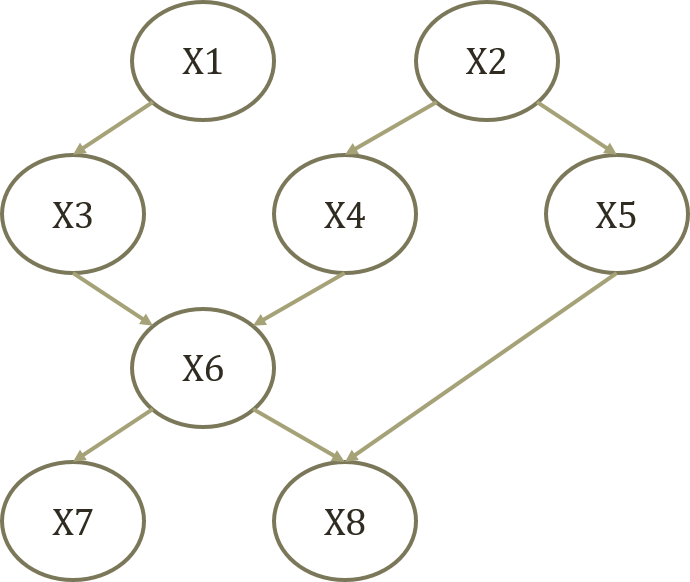
\includegraphics[scale=0.45]{fig7_14.png} 
\caption{베이지안 네트워크에서의 결합 확률 분해 예시}
\label{fig:7-14}
\end{figure} 

예를 들어, 그림 \ref{fig:7-14}의 베이지안 네트워크의 정보를 활용해서 결합 확률을 분해해 보자. 여기서 각 $X_i$는 부모 노드로부터만 직접적인 영향을 받는다. 따라서 이런 영향 관계를 활용하면 다음과 같이 베이지안 네트워크를 분해할 수 있다.  

\begin{eqnarray}
P(X_1,\cdots,X_8) & = & P(X_1) P(X_2) P(X_3|X_1) P(X_4|X_2) P(X_5|X_2) \nonumber\\
& & P(X_6|X_3,X_4) P(X_7|X_6) P(X_8|X_5,X_6) \label{eq:7-14-1}
\end{eqnarray}

또한, 앞서 설명한 d-분해를 결합 확률의 분해에 적용할 수 있으나 여기서 다루지는 않겠다. \\

%정보가 주어진 노드가 있는 베이지안 네트워크에 대해서는 베이즈 볼 알고리즘으로 노드 사이의 영향 관계를 알아내고 이러한 것을 분해 과정에서 활용할 수 있겠다. 한편으로,

%-----------------------------------------------------------------
\subsection{추론}
%-----------------------------------------------------------------

%슬라이드 23%
이제는 베이지안 네트워크에서 나온 결합 함수를 어떻게 활용할 수 있는지 알아보겠다. 먼저 우도의 계산이 있다. 우도(Likelihood)는 우리가 관찰한 값이 실제로 나올 확률을 구한 것이다. 먼저 베이지안 네트워크에 있든 모든 확률 변수를 $X=\{X_1, \cdots, X_N\}$라고 하자. 그러면 그 중에는 이미 증거값(Evidence Value) $x_V$가 주어진 증거 변수(Evidence Variable) $X_V=\{X_{k+1}, \cdots, X_N\}$가 있고, 그 외 나머지 숨은 변수(Hidden Variable) $X_H=\{X_1, \cdots, X_k\}$가 있을 수 있다. 그러면 이미 관찰된 값인 $X_V=x_V$에 한해서 우도를 계산하면 다음과 같다. 
\begin{eqnarray}
P(x_V) & = & \sum_{X_{H}} P(X_{H},x_V) \nonumber \\
& = & \sum_{x_{1}} \cdots  \sum_{x_{k}} P(x_{1}, \cdots x_{k}, x_V) \label{eq:7-15}
\end{eqnarray}
수식 (\ref{eq:7-15})에서는 결합 함수만을 사용하고 있으므로, 우리는 한 번에 우도를 계산할 수 있다. 또한, 이것을 그대로 활용해서 우도함수를 계산할 수도 있다. 파라미터 $\theta$가 조건부 확률값이나 확률 분포의 파라미터 값과 같은 변수의 확률 파라미터라면, 다음과 같이 우도함수를 구할 수 있다.
\begin{eqnarray}
L(\theta) & = & P(x_V|\theta) \nonumber \\
& = & \sum_{X_{H}} P(X_{H},x_V|\theta) \nonumber \\
& = & \sum_{x_{1}} \cdots  \sum_{x_{k}} P(x_{1}, \cdots x_{k}, x_V |\theta) \label{eq:7-15-1}
\end{eqnarray}
우리는 수식 (\ref{eq:7-15-1})의 결과를 최대화하면서 우도함수를 최대화하는 최우추정량(Maximum Likelihood Estimator)을 찾을 수 있다. \\

%슬라이드 24%
다음은 조건부 확률의 계산이다. 앞에서처럼 증거 변수 $X_V$와 숨은 변수 $X_H$가 주어졌을 때, 이번에는 $X_H$를 우리가 알고 싶어하는 확률 변수의 집합인 $Y$와 알지 못해도 상관 없는 변수의 집합인 $Z$로 나누자. 그러면 $Y$의 확률을 다음과 같이 구할 수 있다. 
\begin{eqnarray}
P(Y|x_V) & = & \sum_{z} P(Y,Z=z|x_V) \nonumber \\
& = & \sum_{z} \frac{P(Y,Z=z,x_V)}{P(x_V)} \nonumber \\
& = & \frac{\sum_{z} P(Y,Z=z,x_V)}{\sum_{y} \sum_{z} P(Y=y,Z=z,x_V)} \label{eq:7-16}
\end{eqnarray}
수식 (\ref{eq:7-16})의 결과값은 분자와 분모 모두 결합 함수만을 사용하고 있다. 따라서 결함 함수를 알면 조건부 확률 역시 계산할 수 있다. \\

%슬라이드 25%
마지막은 예측과 진단이다. 앞에서처럼 증거 변수 $X_V$와 숨은 변수 $X_H$, 숨은 변수 중에서 우리가 알고 싶어하는 변수의 집합인 $Y$가 있다. 그렇다면 $Y$의 값으로 가장 적절한 것은 무엇일까? 이것 또한 최대 우도를 찾는 문제이다. 여기서는 $Y$가 그 자체로 확률 변수이므로 각 $Y$별로 조건부 확률값을 직접 구하고 비교해서 가장 큰 확률값을 가지는 $Y^*$를 찾을 수가 있다. 

\begin{equation}
L(Y) = \textrm{max}_{Y} P(Y|x_V), \ \ \ Y^* = \textrm{argmax}_{Y} P(Y|x_V)
\label{eq:7-17}
\end{equation}

이러한 귀납적(a posteriori) 과정은 $Y$가 $x_V$의 영향을 받았다면 $x_V$의 결과로서 $Y$를 예측(Prediction)한 것이 되며, $Y$가 $x_V$에 영향을 준 것이라면 $x_V$의 원인인 $Y$를 진단(Diagnosis)한 것이 된다.


%-----------------------------------------------------------------
\subsection{변수 축소}
%-----------------------------------------------------------------

이번에는 베이지안 네트워크에서의 결합 확률을 보다 더 빨리 계산할 수 있는 방법에 대해서 생각해 보도록 하겠다. 설명을 쉽게 하기 위해서 section 2.1에서 사용했던 베이지안 네트워크 예시를 다시 사용할 것이다. \\  

\begin{figure}[ht] \centering 
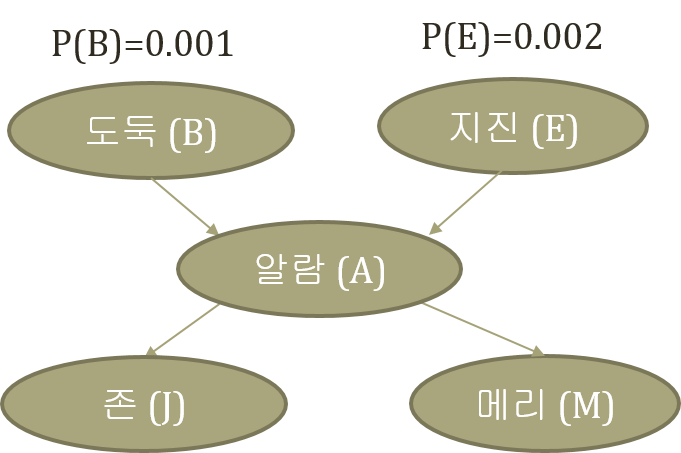
\includegraphics[scale=0.45]{fig7_8.png} 
\caption{베이지안 네트워크 예시}
\label{fig:7-17}
\end{figure} 

\begin{figure}[ht] \centering 
\parbox[t]{3cm}
{
\begin{tabular}{|c|c|c|}
  \hline
  도둑($B$) & 지진($E$) & $P(A|B,E)$ \\
  \hline
  true & true & 0.95 \\
  \hline
  true & false & 0.94 \\
  \hline
  false & true & 0.29 \\
  \hline
  false & false & 0.001 \\
  \hline
\end{tabular}
} \hspace{3cm}
\parbox[t]{5cm}
{
\begin{tabular}{|c|c|c|}
  \hline
  알람($A$) & $P(J|A)$ & $P(M|A)$ \\
  \hline
  true & 0.90 & 0.70 \\
  \hline
  false & 0.05 & 0.01 \\
  \hline
\end{tabular}
}
\caption{조건부 확률 표}
\label{fig:7-16}
\end{figure} 

이제 도둑이 들었고, 알람이 울렸으며, 메리가 알람이 울렸다는 사실을 나에게 전화로 알려왔다고 하자. 이러한 상황이 발생할 확률은 어떻게 될까? 이것을 다음과 같이 결합 확률의 합으로 표현할 수 있다. 
\begin{eqnarray}
P(A=\textrm{true}, B=\textrm{true}, M=\textrm{true}) \ \ \ \ \ \ \ \ \ \ \ \ \ \ \ \ \ \ \ \ \ \ \ \ \  \nonumber  \\
= \sum_{J} \sum_{E} P(A=\textrm{true},B=\textrm{true},E,J,M=\textrm{true}) \label{eq:7-17-1}
\end{eqnarray}
그리고 section 3.1에서 언급한 결합 확률의 분해를 사용하면, 다음과 같이 식을 전개할 수 있다. 
\begin{eqnarray}
P(A=\textrm{true}, B=\textrm{true}, M=\textrm{true}) = \sum_{J} \sum_{E} P(J|A=\textrm{true}) \ \ \ \ \ \  \ \ \ \ \nonumber  \\
\times \ P(M|A=\textrm{true}) P(A=\textrm{true}|B=\textrm{true},E) P(E) P(B)   \label{eq:7-18} 
\end{eqnarray}
수식 \ref{eq:7-18}의 확률값을 계산하기 위해서는 $E$와 $J$의 경우의 수를 곱한 만큼의 결합 확률값이 필요하며, 각각의 결합 확률값을 구하기 위해서는 베이지안 네트워크의 확률 변수의 개수에 1을 뺀 만큼의 곱셈이 또 필요하다. 이처럼 최종 확률값을 구하기 위해서는 수많은 곱셈이 필요하며, 확률 변수의 개수가 많아질수록 이런 방식으로 계산하는 것은 크게 비효율적이게 된다. 이러한 상황을 개선하기 위해서 $E$, $J$와 관계없는 확률을 시그마 밖으로 빼내어서 앞으로 가져오자. 그러면 식을 다음과 같이 바꿀 수 있다. 
\begin{eqnarray}
P(A=\textrm{true}, B=\textrm{true}, M=\textrm{true}) = P(B) P(M|A=\textrm{true})  \ \ \ \ \ \  \ \ \ \ \nonumber  \\
 \times \  \sum_{J} P(J|A=\textrm{true}) \sum_{E} P(A=\textrm{true}|B=\textrm{true},E) P(E) \label{eq:7-19} 
\end{eqnarray}
이제는 각 $J$에 대해서 $P(J|A=\textrm{true})$값을 구해서 더한 값과 각 $E$에 대해서 $P(A=\textrm{true}|B=\textrm{true},E)P(E)$값을 구해서 더한 값을 $P(B) P(M|A=\textrm{true})$에 곱하는 것으로 우리가 원하는 확률값을 이전과 비교했을 때 보다 효율적으로 구할 수 있다. \\

이번에는 존과 메리로부터 동시에 전화가 왔다고 하자. 그렇다면 지진이 발생했을 확률은 어떻게 될까? 여기서는 $J$, $M$이 각각 $j(\textrm{true})$, $m(\textrm{true})$로 고정된 상황에서 $E$가 $e(\textrm{true})$일 확률을 계산할 것이다. 여기서 처음으로 우리가 해야 할 일은 조건부 확률의 정의에 따라서 그것을 분해하는 것이다. 여기서는 $J=j$, $M=m$이 주어졌으므로 $1/P(J=j, M=m)$은 상수이며, 이것을 $\alpha$로 두겠다. 그러면 다음과 같이 수식을 전개할 수 있다.
\begin{equation}
P(E=e | J=j, M=m) = \alpha P(E=e, J=j, M=m) 
\label{eq:7-20-1}
\end{equation}
다음으로, 수식 (\ref{eq:7-20-1})을 결합 함수의 합으로 나타내야 한다. 이 과정에서는 앞에서 설명한 것처럼 베이지안 네트워크에서 찾을 수 있는 노드 사이의 연관 관계를 활용해서 결합 함수를 적절히 분해할 수 있어야 한다. 
\begin{eqnarray}
P(E=e, J=j, M=m) \ \ \ \ \ \  \ \ \ \ \ \ \ \ \ \  \ \ \ \ \ \ \ \ \ \ \ \ \ \ \ \ \ \ \ \ \ \ \ \ \ \  \ \ \ \ \ \nonumber \\
= \sum_{B} \sum_{A} P(J=j|A) P(M=m|A) P(A|B,E=e) P(E=e) P(B) \label{eq:7-20}
\end{eqnarray}
한편, 각 변수 사이의 직접적인 부모 노드가 자식 노드보다 먼저 올 수 있도록 나열해야 한다. 사실 베이지안 네트워크는 비순환 방향 그래프이므로 이러한 위상적 순서로 노드를 나열하는 방법이 반드시 존재한다. 그리고 시그마 기호가 더하는 변수와 관련이 없는 항을 시그마 기호 밖으로 빼내주어야 한다. 
\begin{equation}
\alpha P(E=e) \sum_{B} P(B) \sum_{A} P(A|B,E=e) P(J=j|A) P(M=m|A)
\label{eq:7-21}
\end{equation}
여기서부터는 주어진 변수와 확률값을 가진 P의 의미가 계산 과정에서 계속해서 희석되므로, P를 f로 바꾸어서 다음과 같이 식을 전개하도록 하겠다. 
\begin{equation}
\alpha f_{E}(e) \sum_{b} f_{B}(b) \sum_{a} f_{A}(a,b,e) f_{J}(a) f_{M}(a)
\label{eq:7-23}
\end{equation}
이제 함수 들을 둘씩 서로 곱하면서 수식을 점점 축소해 나가겠다. $f_{J}(a)$와 $f_{M}(a)$을 곱한 함수를 $f_{JM}(a)$라고 하자. 그러면 식을 다음처럼 전개할 수 있다. 
\begin{equation}
\alpha f_{E}(e) \sum_{b} f_{B}(b) \sum_{a} f_{A}(a,b,e) f_{JM}(a)
\label{eq:7-24}
\end{equation}
그림 \ref{fig:7-19}의 표에서 각각의 $a$에 대한 $f_{JM}(a)$의 값을 확인할 수 있다.  
 
\begin{figure}[ht] \centering 
\begin{tabular}{|c|c|c|c|c|c|}
  \hline
  알람($a$) & $f_{J}(a)$ &  & $f_{M}(a)$ &  & $f_{JM}(a)$   \\
  \cline{1-2} \cline{4-4} \cline{6-6}
  true & 0.90 & $\times$ & 0.70 & $=$ & 0.63 \\
  \cline{1-2} \cline{4-4} \cline{6-6}
  false & 0.05 &  & 0.01 &  & 0.0005\\
  \hline
\end{tabular}
\caption{$f_{JM}(a)$ 계산 표}
\label{fig:7-19}
\end{figure} 
다음으로, $f_{A}(a,b,e)$와 $f_{JM}(a)$를 곱한 함수를 $f_{AJM}(a,b,e)$라고 하자. 그러면 식을 다음과 같이 전개할 수 있다.
\begin{equation}
\alpha f_{E}(e) \sum_{b} f_{B}(b) \sum_{a} f_{AJM}(a,b,e)
\label{eq:7-25}
\end{equation}
그림 \ref{fig:7-21}의 표에서 각각의 $a$, $b$에 대한 $f_{AJM}(a,b,e)$의 값을 확인할 수 있다. ($e=\textrm{true}$로 값이 정해져 있다는 사실에 주의하자.) 

\begin{figure}[ht] \centering 
\begin{tabular}{|c|c|c|c|}
  \hline
  알람($a$) & 도둑($b$) & $f_{AJM}(a,b,e)$\\
  \hline
  true & true & 0.95$\times$0.63 \\
  \hline
  true & false & 0.29$\times$0.63 \\
  \hline
  false & true & (1-0.95)$\times$0.0005 \\
  \hline
  false & false & (1-0.29)$\times$0.0005 \\
  \hline
\end{tabular}
\caption{$f_{AJM}(a,b,e)$ 계산 표}
\label{fig:7-21}
\end{figure} 
\noindent 다음으로, $f_{AJM}(a,b,e)$를 모든 $a$의 경우에 대해서 더한 함수를 $f_{\bar{A}JM}(b,e)$라 하겠다.
\begin{equation}
\alpha f_{E}(e) \sum_{b} f_{B}(b) f_{\bar{A}JM}(b,e)
\label{eq:7-26}
\end{equation}
그리고 $f_{B}(b)$와 $f_{\bar{A}JM}(b,e)$를 곱한 함수를 $f_{\bar{A}BJM}(b,e)$라고 하겠다.
\begin{equation}
\alpha f_{E}(e) \sum_{b}  f_{\bar{A}BJM}(b,e)
\label{eq:7-27}
\end{equation}
그림 \ref{fig:7-23}의 표에서 $b$가 true, false일 경우에 각각의 $f_{\bar{A}BJM}(b,e)$의 값을 확인할 수 있다.

\begin{figure}[ht] \centering
\begin{tabular}{|c|c|c|}
  \hline
  도둑($b$)  &  $f_{\bar{A}BJM}(b,e)$\\
  \hline
  true & 0.95$\times$0.63 \ + \ (1-0.95)$\times$0.0005 \ = \ 0.599\\ 
  \hline
  false & 0.29$\times$0.63 \ + \ (1-0.29)$\times$0.0005 \ = \ 0.183\\ 
  \hline
\end{tabular}
\caption{$f_{\bar{A}BJM}(b,e)$ 계산 표}
\label{fig:7-23}
\end{figure} 

\noindent 다음으로, $f_{\bar{A}BJM}(b,e)$를 모든 $b$의 경우에 대해서 더한 함수를 $f_{\bar{A}\bar{B}JM}(e)$라 하겠다.
\begin{equation}
\alpha f_{E}(e) f_{\bar{A}\bar{B}JM}(e)
\label{eq:7-28}
\end{equation}
그리고 $f_{E}(e)$와 $f_{\bar{A}\bar{B}JM}(e)$를 곱한 함수를 $f_{\bar{A}BJM}(b,e)$라고 하겠다.
\begin{equation}
\alpha f_{\bar{A}\bar{B}EJM}(e)
\label{eq:7-29}
\end{equation}
그러면 $f_{\bar{A}\bar{B}EJM}(e)$의 값을 다음과 같이 계산할 수 있다.  
\begin{equation}
f_{\bar{A}\bar{B}EJM}(e) = 0.001*0.599+(1-0.001)*0.183 = 0.183
\label{eq:7-30}
\end{equation}
따라서 우리가 원하는 확률값은 수식 (\ref{eq:7-31})와 같다.
\begin{equation}
P(E=e | J=j, M=m) = \alpha \cdot 0.183
\label{eq:7-31}
\end{equation}

이런 식으로 주변화 과정으로 변수의 개수를 줄여나가는 일련의 과정을 변수 축소(Variable Elimination)라고 한다. 변수 축소를 활용하면 조건부 확률을 쉽고 빠르게, 체계적으로 계산할 수 있다. 그러나 한 가지 명심해야 할 것은, 각각의 경우에 대한 결합 확률값을 구해서 모두 더하는 방법 대신에 변수 축소를 사용해서 확률값을 계산하더라도 이론적으로는 여전히 지수적 시간 복잡도(Exponential Time Complexity)를 나타낸다는 것이다. 

%-----------------------------------------------------------------
\section{접합 트리 알고리즘}
%-----------------------------------------------------------------
%-----------------------------------------------------------------
\subsection{신뢰 전파}
%-----------------------------------------------------------------
%슬라이드 33%
이제는 이전보다 더욱 복잡한 네트워크를 분석할 수 있는 접합 트리 알고리즘을 다루도록 하겠다. 그러나 접합 트리 알고리즘이 왜 필요한지,  어떻게 작동하는지를 제대로 이해하기 위해서는 잠재 함수나 클릭과 같은 기본 개념과 특정 베이지안 네트워크에 적용할 수 있는 신뢰 전파를 이해하고 있어야 한다. \\

잠재 함수(Potential Function)는 확률 분포 함수는 아니지만 정규화 과정을 거치고 나면 확률 분포함수로 기능할 수 있는 함수를 말하며, 베이지안 네트워크에서의 신뢰 전파를 이해하기 위해서 사용한다. 잠재 함수를 이해하기 위해서 그림 \ref{fig:7-24}의 선형 베이지안 네트워크를 놓고 한 번 생각해 보도록 하겠다. \\

\begin{figure}[ht] \centering 

\includegraphics[scale=0.45]{fig7_18.png} 
\caption{선형 베이지안 네트워크}
\label{fig:7-24}
\end{figure} 

\noindent 여기에는 $A$, $B$, $C$, $D$의 네 개의 노드가 있으며, 세 개의 아크가 노드를 차례대로 연결하고 있다. 여러분은 이전에 배운 내용대로 결합 함수 $P(A,B,C,D)$를 다음과 같이 분해할 수 있을 것이다.
\begin{equation}
P(A,B,C,D) = P(A|B) P(B|C) P(C|D) P(D)
\label{eq:7-32}
\end{equation} \\

이 그래프를 클릭(Clique)과 분리기(Separator)로 이루어진 클릭 그래프(Clique Graph)로 나타내어 보자. 여기서 클릭이란 부분 그래프의 하나로서, 그것에 포함되어 있는 모든 두 노드가 아크로 연결되어 있어야 한다. 그림 \ref{fig:7-24}의 그래프에서는 $A$와 $B$, $B$와 $C$, $C$와 $D$가 서로 아크로 연결되어 있으므로 이것들은 모두 노드가 두 개인 클릭이라고 할 수 있다. 따라서 이것들을 각각 $AB$, $BC$, $CD$로 묶어주겠다. 또한, 서로 다른 두 클릭이 같은 노드를 가질 수도 있으며, 여기서의 두 클릭을 아크로 연결하고 거기에다 두 클릭이 공통으로 가지고 있는 노드가 무엇인지에 대한 정보를 넣을 수 있다. 이러한 정보를 포함하는 클릭과 클릭 사이의 연결을 분리기라고 한다. 그림 \ref{fig:7-24}의 선형 베이지안 네트워크는 그림 \ref{fig:7-25}의 클릭 그래프로 나타낼 수 있다. \\   

\begin{figure}[ht] \centering 
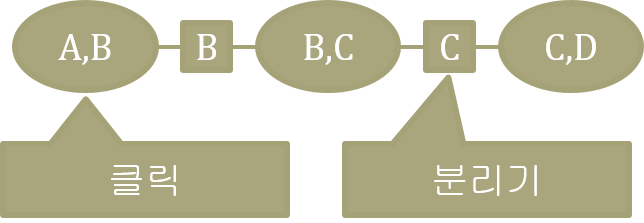
\includegraphics[scale=0.45]{fig7_19.png} 
\caption{선형 베이지안 네트워크의 클릭 그래프}
\label{fig:7-25}
\end{figure} 

여기서 우리는 각 클릭에 잠재 함수 $\psi(A,B)$, $\psi(B,C)$, $\psi(C,D)$를 설정하였으며, 같은 식으로 각 분리기에 대해서도 잠재 함수 $\phi(B)$, $\phi(C)$를 정의할 수가 있다. 하지만 지금까지는 잠재 함수에 어떠한 의미도 부여하지 않았으며, 이제부터 잠재 함수가 가져야 하는 성질을 하나하나 설명해 나가도록 하겠다. 먼저 잠재 함수는 클릭에 대한 모든 잠재 함수를 곱한 것에 분리기에 대한 모든 잠재 함수를 곱한 것을 나눈 함수는 처음 베이지안 네트워크의 결합 함수와 같아야 한다. 이것을 수식으로 나타내면 다음과 같다. 
\begin{equation}
P(A,B,C,D) = P(U) = \frac{ \prod_{N} \psi(N) }{ \prod_{L} \phi(L) } = \frac{\psi(A,B)\psi(B,C)\psi(C,D) }{ \phi(B) \phi(C) }
\label{eq:7-33}
\end{equation} 
따라서 처음에 수식 (\ref{eq:7-32})에서 $P(A,B,C,D)$를 분해한 것을 바탕으로 생각해 보면 $\phi(B)$와 $\phi(B)$을 모두 1로 두고 각각의 $\psi$값을 다음과 같이 정의할 수 있다. 
\begin{equation}
\psi(A,B) = P(A|B), \ \psi(B,C) = P(B|C), \ \psi(C,D) = P(C|D) P(D)
\label{eq:7-34}
\end{equation} 
또는 $\phi(B)=P(B)$, $\phi(C)=P(C)$로 두고 각각의 $\psi$값을 다음과 같이 정의할 수도 있다.  
\begin{equation}
\psi(A,B) = P(A, B), \ \psi(B,C) = P(B, C), \ \psi(C,D) = P(C, D)
\label{eq:7-35}
\end{equation} 
여기서 수식 (\ref{eq:7-34})에서는 조건부 확률을, 수식 (\ref{eq:7-35})에서는 결합 확률을 사용했으나, 두 경우 모두 $\psi(A,B)\psi(B,C)\psi(C,D)$에 $\phi(B) \phi(C)$를 나눈 식이 $P(A,B,C,D)$과 일치하므로 처음에 말한 조건을 만족시킨다. 그러나 우리가 가진 정보는 주로 조건부 확률에 대한 정보이므로, 일반적으로는 수식 (\ref{eq:7-35})의 정의보다는 수식 (\ref{eq:7-34})의 정의를 사용하는 것이 이후의 계산에 있어서 편한 길이 된다. \\

또한, 주변화를 적용해서 구성한 확률 변수의 부분집합에 대해서도 잠재 함수를 정할 수 있다. 확률 변수의 부분집합 $W$가 있을 때 그것의 잠재 함수 $\psi(W)$는 $W$에 속한 모든 $V$에 대해서 잠재 함수를 더한 것과 같다. 그리고 이것을 수식으로 나타내면 다음과 같다.  
\begin{equation}
\psi(W) = \sum_{V \in W} \psi(V)
\label{eq:7-36}
\end{equation} \\  

%슬라이드 34%
이제 트리 구조를 가진 클릭 그래프에 적용할 수 있는 흡수(Absorption)에 대해서 알아보도록 하겠다. 이것은 데이터 구조의 관점에서 확률을 추측할 수 있도록 돕는다. 예를 들어, 우리가 앞서 그림 \ref{fig:7-25}의 클릭 그래프에서 $\psi(A,B)$, $\psi(B,C)$와 $\phi(B)$를 수식 (\ref{eq:7-35})에서처럼 각각 $P(A, B)$, $P(B, C)$와 $P(B)$로 정했다고 하자. 그러면 $P(B)$를 다음과 같이 클릭과 분리기를 사용해서 세 종류의 수식으로 나타낼 수 있게 된다.  
\begin{equation}
P(B) = \sum_{A} \psi(A,B) = \sum_{C} \psi(B,C) = \phi(B)
\label{eq:7-37}
\end{equation} 
이 때, 관측에 의해서 $\psi(A,B)$, $\psi(B,C)$, $\phi(B)$ 중 하나의 값을 새로 갱신해 준다면 그에 따라서 $P(B)$의 값이 변하게 된다. 그리고 수식 (\ref{eq:7-37})의 관계에 따라 다른 클릭이나 분리기의 값 또한 변하게 된다. 이렇게 새로이 관측한 정보가 그것의 주변으로 전파하는 것을 신뢰 전파(Belief Propagation)라고 한다. 또한, 수식 (\ref{eq:7-37})과 같은 클릭이나 분리기 사이의 관계는 그것들 중 어느 하나의 값이 바뀌더라도 변하지 않으며, 이를 흡수 규칙(Absorption Rule) 또는 갱신 규칙(Update Rule)이라고 한다.     \\

그림 \ref{fig:7-25}의 클릭 그래프로 신뢰 전파가 어떤 식으로 이루어지는지를 구체적으로 살펴보도록 하겠다. 먼저 $\psi(A,B)$가 관측에 의해서 $\psi^{*}(A,B)$로 바뀌었다고 하자. 그러면 $\phi(B)$와 $\psi(B,C)$도 $\phi^{*}(B)$와 $\psi^{*}(B,C)$로 바꿔줘야 하지만, 이러한 변화는 어디까지나 흡수 규칙에 따라서 이루어져야 한다. 먼저 수식 (\ref{eq:7-37})에 따라 $\phi^{*}(B)$는 다음과 같이 정해진다.  
\begin{equation}
\phi^{*}(B) = \sum_{A} \psi^{*}(A,B)
\label{eq:7-38}
\end{equation}
또한, $\psi^{*}(B,C)$의 값은 다음과 같다. 
\begin{equation}
\psi^{*}(B,C) = \psi(B,C) \ \frac{\phi^{*}(B)}{\phi(B)}
\label{eq:7-39}
\end{equation}
그러나 수식 (\ref{eq:7-39})이 흡수 규칙을 따르는지는 아직 확인되지 않았다. 이것을 보이기 위해서는 $\sum_{C} \psi^{*}(B,C)$가 $\sum_{A} \psi^{*}(A,B)$ 또는 $\phi^{*}(B)$와 같다는 사실을 보이는 것으로 충분하다. 다음 수식으로 이러한 사실을 증명할 수 있다.  
\begin{eqnarray}
\sum_{C} \psi^{*}(B,C) & = & \sum_{C} \psi(B,C) \ \frac{\phi^{*}(B)}{\phi(B)}  = \frac{\phi^{*}(B)}{\phi(B)} \sum_{C} \psi(B,C) \nonumber \\
& = & \frac{\phi^{*}(B)}{\phi(B)} \ \phi(B) = \phi^{*}(B) \label{eq:7-40}
\end{eqnarray}
이렇게 신뢰 전파가 클릭 $A,B$에서 시작해서 분리기 $B$, 클릭 $B,C$로 새로 갱신한 정보가 계속 전파되는 과정을 확인할 수 있다. 이러한 신뢰 전파의 과정을 계속해서 진행해 나간다면 분리기 $C$, 클릭 $C,D$까지 계속하면서 정보가 순차적으로 퍼지게 된다. \\

%슬라이드 35%
이제 신뢰 전파의 반복 과정에 대해서 보다 자세히 알아보도록 하겠다. 먼저 다음과 같이 세 개의 노드와 두 개의 아크로 이루어진 앞에서의 예시와 비교했을 때 더욱 단순한 형태의 베이지안 네트워크가 있다고 하겠다.  \\

\begin{figure}[ht] \centering 

\includegraphics[scale=0.8]{fig7_20.png} 
\caption{베이지안 네트워크}
\label{fig:7-22}
\end{figure} 

\noindent 그림 \ref{fig:7-22}의 클릭 그래프는 그림 \ref{fig:7-26}에서처럼 클릭 $AB$, $BC$와 분리기 $B$로 구성된다. \\

\begin{figure}[ht] \centering 
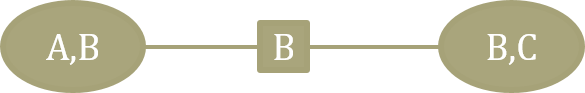
\includegraphics[scale=0.8]{fig7_21.png} 
\caption{클릭 그래프}
\label{fig:7-26}
\end{figure} 

신뢰 전파를 진행하기 위해서 우선 각 클릭과 분리기의 잠재 함수를 다음과 같이 정하였다.
\begin{equation}
\psi(A,B) = P(A|B), \ \psi(B,C) = P(B|C)P(C) = P(B,C), \ \phi(B) = 1
\label{eq:7-41}
\end{equation} 
여기서 그림 \ref{fig:7-26}의 클릭 그래프는 그림 \ref{fig:7-25}의 클릭 그래프에서처럼 클릭과 분리기가 번갈아가며 연결되어 있는 구조로 되어 있으므로, 신뢰 전파 과정에서 수식 (\ref{eq:7-38})과 수식 (\ref{eq:7-39})를 그대로 적용할 수 있다. 따라서 새로운 $\phi^{*}(B)$를 다음과 같이 계산할 수 있다. 
\begin{equation}
\phi^{*}(B) = \sum_{A} \psi(A,B) = 1
\label{eq:7-42}
\end{equation} 
그리고 갱신된 $\phi^{*}(B)$를 활용해서 $\psi^{*}(B,C)$를 다음과 같이 계산할 수 있다. 
\begin{equation}
\psi^{*}(B,C) = \psi(B,C) \ \frac{\phi^{*}(B)}{\phi(B)} = P(B,C) \ \frac{1}{1} = P(B,C)
\label{eq:7-43}
\end{equation} 
다음으로, 그래프 구조상 클릭 $B,C$에는 자식이 없으므로 분리기 $B$로 되돌아가서 $\psi^{*}(B,C)$로 새로운 $\phi^{**}(B)$를 다음과 같이 계산할 수 있다. 
\begin{equation}
\phi^{**}(B) = \sum_{C} \psi(B,C) = \sum_{C} P(B,C) = P(B)
\label{eq:7-44}
\end{equation} 
그리고 $\phi^{**}(B)$를 활용해서 분리기 $B$의 왼쪽에 있는 클릭 $A,B$의 잠재 함수인 $\psi^{*}(A,B)$를 계산하면 다음과 같이 나온다. 
\begin{equation}
\psi^{*}(A,B) = \psi(A,B) \ \frac{\phi^{**}(B)}{\phi^{*}(B)} = \frac{P(A|B)P(B)}{1} = P(A,B)
\label{eq:7-45}
\end{equation} 
마지막으로, 이렇게 갱신된 $\psi^{*}(A,B)$를 활용해서 또 다시 새로운 $\phi^{***}(B)$를 계산하면 분리기 $B$의 잠재 함수는 다음과 같이 나온다. 
\begin{equation}
\phi^{***}(B) = \sum_{A} \psi^{*}(A,B) = \sum_{A} P(A,B) = P(B)
\label{eq:7-46}
\end{equation} 
이 뒤에는 계속해서 신뢰 전파 과정을 적용하더라도 잠재 함수가 더 이상 변하지 않으므로 전체 과정은 끝난 것이 된다. 따라서 $\phi^{***}(B)$의 값이 $P(B)$의 값이라고 생각할 수 있다. 한편, 이러한 신뢰 전파에서 처음에는 수식 (\ref{eq:7-41})과 같이 조건부 확률의 형태로 클릭의 잠재 함수가 주어졌으나 이후의 과정에서 클릭의 잠재 함수가 결합 확률과 같게 되는 것을 확인할 수 있다. \\

이번에는 신뢰 전파로 $A$와 $C$의 값이 $A=a$, $C=c$로 주어져 있다는 조건 아래에서의 $B$의 조건부 확률 분포 함수를 계산해보도록 하겠다. 처음 잠재 함수의 정의는 앞에서와 같이 수식 (\ref{eq:7-41})의 그것으로 정하였다. 또한, 이후의 과정 역시 잠재 함수인 $\phi(B)$, $\psi(B,C)$, $\psi(A,B)$를 앞에서와 같은 순서로 차례대로 갱신하는 것이 된다. 먼저 $\phi^{*}(B)$의 값이 다음과 같이 새로이 정해진다.  
\begin{equation}
\phi^{*}(B) = \sum_{A=a} \psi(A,B) = \psi(A=a,B) = P(A=a|B)
\label{eq:7-47}
\end{equation} 
여기서 $A=a$라는 것이 사전에 주어져 있으므로 결합 함수를 모든 $A$에 대해서 합하는 주변화의 적용에 있어서는 $A=a$인 경우만을 반영해 주었다. 이런 식으로 앞으로도 $A=a$, $C=c$라는 사전 정보를 잘 반영하면서 신뢰 전파를 진행할 것이다. 다음으로 클릭 $B,C$에 대한 잠재 함수 $\psi^{*}(B,C=c)$가 다음처럼 갱신된다. 
\begin{eqnarray}
\psi^{*}(B,C=c) & = & \psi(B,C=c) \ \frac{\phi^{*}(B)}{\phi(B)} \nonumber \\
& = & P(B|C=c)P(C=c) \ \frac{P(A=a|B)}{1} \nonumber \\
& = & P(B|C=c)P(C=c)P(A=a|B) \label{eq:7-48}
\end{eqnarray}
이것을 활용해서 $\phi^{**}(B)$를 다시 한 번 갱신할 수 있다. 
\begin{eqnarray}
\phi^{**}(B) & = & \sum_{C=c} \psi(B,C)  \nonumber \\
& = & \psi(B,C=c) = P(B|C=c)P(C=c)P(A=a|B)
\label{eq:7-49}
\end{eqnarray} 
다음으로 $\phi^{**}(B)$으로 $\psi^{*}(A=a,B)$를 다음과 같이 계산할 수 있다. 
\begin{eqnarray}
\psi^{*}(A=a,B) & = & \psi(A=a,B) \ \frac{\phi^{**}(B)}{\phi^{*}(B)}  \nonumber \\
& = & P(A=a|B) \frac{P(B|C=c)P(C=c)P(A=a|B)}{P(A=a|B)} \nonumber \\
& = & P(A=a|B)P(B|C=c)P(C=c) \label{eq:7-50}
\end{eqnarray} 
마지막으로 새로 만들어진 $\psi^{*}(A=a,B)$를 다시 $A$에 대해서 주변화해주면 $\phi^{***}(B)$를 갱신할 수 있으며, 그것은 다음과 같이 나온다. 
\begin{equation}
\phi^{***}(B) = \sum_{A=a} \psi^{*}(A,B) = \psi^{*}(A=a,B) = P(A=a|B)P(B|C=c)P(C=c)
\label{eq:7-51}
\end{equation}
이제는 더 이상 진행하더라도 새로운 잠재 함수에는 변화가 없게 되므로 신뢰 전파 과정은 여기서 끝난다. 그리고 마지막에 나온 $\phi^{***}(B)$을 계산해서 조건부 확률인 $P(A|B,C)$를 구할 수 있다. \\

우리는 이런 식으로 신뢰 전파 과정을 거대한 규모의 베이지안 네트워크에 적용해서 보다 효율적으로 확률값을 계산할 수 있다. 그러나 여기서 한 가지 명심할 것은 신뢰 전파를 사용할 수 있는 베이지안 네트워크는 그것의 클릭 그래프 구조가 트리로 한정되어 있다는 것이다. 일반적인 베이지안 네트워크에 대해서 흡수와 같은 규칙을 적용할 수 있도록 하려면 새로운 알고리즘이 필요하다.  


%-----------------------------------------------------------------
\subsection{접합 트리 알고리즘}
%-----------------------------------------------------------------

앞서 설명한 신뢰 전파 과정은 클릭 그래프가 트리인 경우에만 적용할 수 있었다. 이는 트리 구조에서는 두 노드를 연결하는 경로가 정확히 하나만 존재하기 때문에 정보가 특정 지점에서 다른 지점으로 도달하기 위해서는 반드시 정해진 하나의 경로만을 거쳐야 하기 때문이다. 그러나 클릭 그래프에 사이클이 있다면 두 개의 클릭이나 분리기를 연결하는 경로가 여러 개가 나타날 수 있기 때문에 더 이상 신뢰 전파와 같은 식으로 접근할 수는 없다.  






\end{document}
